\documentclass[11pt]{article}

\usepackage[T1]{fontenc}
\usepackage[utf8]{inputenc}
\usepackage[margin=1in]{geometry}
\usepackage{amsmath,amssymb}
\usepackage{graphicx}
\usepackage{booktabs}
\usepackage{siunitx}
\usepackage{tabularx}
\usepackage[hidelinks]{hyperref}

\sisetup{separate-uncertainty=true}
\graphicspath{{figures/}}

\renewcommand{\thesection}{S\arabic{section}}
\renewcommand{\thetable}{S\arabic{table}}
\renewcommand{\thefigure}{S\arabic{figure}}
\renewcommand{\theequation}{S\arabic{equation}}

\title{Supplementary Information for:\\
\emph{Revisiting Hall--Petch strengthening in FCC high-entropy alloys: best practices for building and auditing machine-learning strength models}}
\author{M.~Mulukutla, S.~P.~Padhy, W.~Xu, B.~P.~Sahu, I.~Karaman, R.~Arr\'{o}yave}
\date{}

\begin{document}
\maketitle
\tableofcontents

% ============================================================
\section{Exploratory data analysis}
\label{si:eda}

\subsection{Sample provenance and synthesis}

The 94 alloys analyzed in this work come from two Bayesian-optimization (BO) campaigns conducted at Texas A\&M University under the BIRDSHOT initiative within the ARL HTMDEC program, building on an earlier six-element campaign that established the BIRDSHOT closed-loop workflow~\cite{Mulukutla2024BIRDSHOT,Hastings2025FCC}.
Figure~\ref{fig:synthesis_verification} documents representative synthesis-verification data, and Figure~\ref{fig:provenance} summarizes design-space coverage.

The first contributing campaign (batches BBA, BBB, BBC; 34 alloys, ${\sim}37\%$ of the dataset) extended the design space to eight elements (Al--Co--Cr--Cu--Fe--Mn--Ni--V) under a single FCC phase-stability constraint. CALPHAD screening (Thermo-Calc TCHEA6/7) retained compositions with FCC fraction ${\geq}0.99$ at both 700 and 950~\si{\degreeCelsius}, yielding ${\sim}27\,000$ feasible alloys. An initial diversity-balanced batch from $k$-medoids clustering was followed by EHVI-driven iterations over Gaussian-process surrogates. Thermomechanical processing was held fixed (60\% cold reduction; recrystallization at 950~\si{\degreeCelsius} for 0.5~h; water quench), so the BBA/BBB/BBC alloys vary only in chemistry.
The campaign design, feasibility-aware acquisition function, and full synthesis record (48 alloys over the three iterations, including the $\sigma$-phase failures that the present single-phase dataset excludes) are documented in the companion BRAVE paper~\cite{Mulukutla2026BRAVE}.

The second contributing campaign (batches CBA, CBB, CBC; 59 alloys, ${\sim}63\%$) is a microstructure-aware BO over a six-element Co--Cr--Fe--Mn--Ni--V subspace ($c_\text{Al} = c_\text{Cu} = 0$ by design). Cold work, recrystallization temperature, and hold time enter as design variables alongside composition, spanning $c_\text{cw} \in \{40, 50, 60\}\%$, $T_\text{rx}$ from 675 to 1250~\si{\degreeCelsius}, and hold times of $\{1, 2, 4, 8\}$~h. The resulting alloys span a wide range of grain sizes at nominally identical compositions, supplying the within-composition microstructural variation that underpins the within-replicate Hall--Petch analysis of Section~\ref{si:premodel}.

All ingots ($\sim$30--35~g) were produced by vacuum arc melting (Edmund B\"{u}hler AM~200) from $>99.9$~wt.\% elemental precursors under high-purity Ar, with 7--10 flip-remelts and mass-loss monitoring (ingots exceeding 0.5\% loss were reprocessed). Each ingot was homogenized for 24~h at 950--1150~\si{\degreeCelsius}, cold-rolled to the campaign-specific reduction, recrystallized under controlled conditions, and water-quenched. Realized compositions were verified by EDS (15 points per ingot); the mean ingot-level deviation from the BO target was 0.4--0.6~at.\%, with 90--99\% of measurements within 1~at.\% of nominal~\cite{Mulukutla2024BIRDSHOT}. Wire-EDM was used to extract miniaturized SS-3 tensile specimens, nanoindentation coupons, and coupons for SEM/EBSD/EDS/XRD/Vickers measurements.

\begin{figure}[htb]
  \centering
  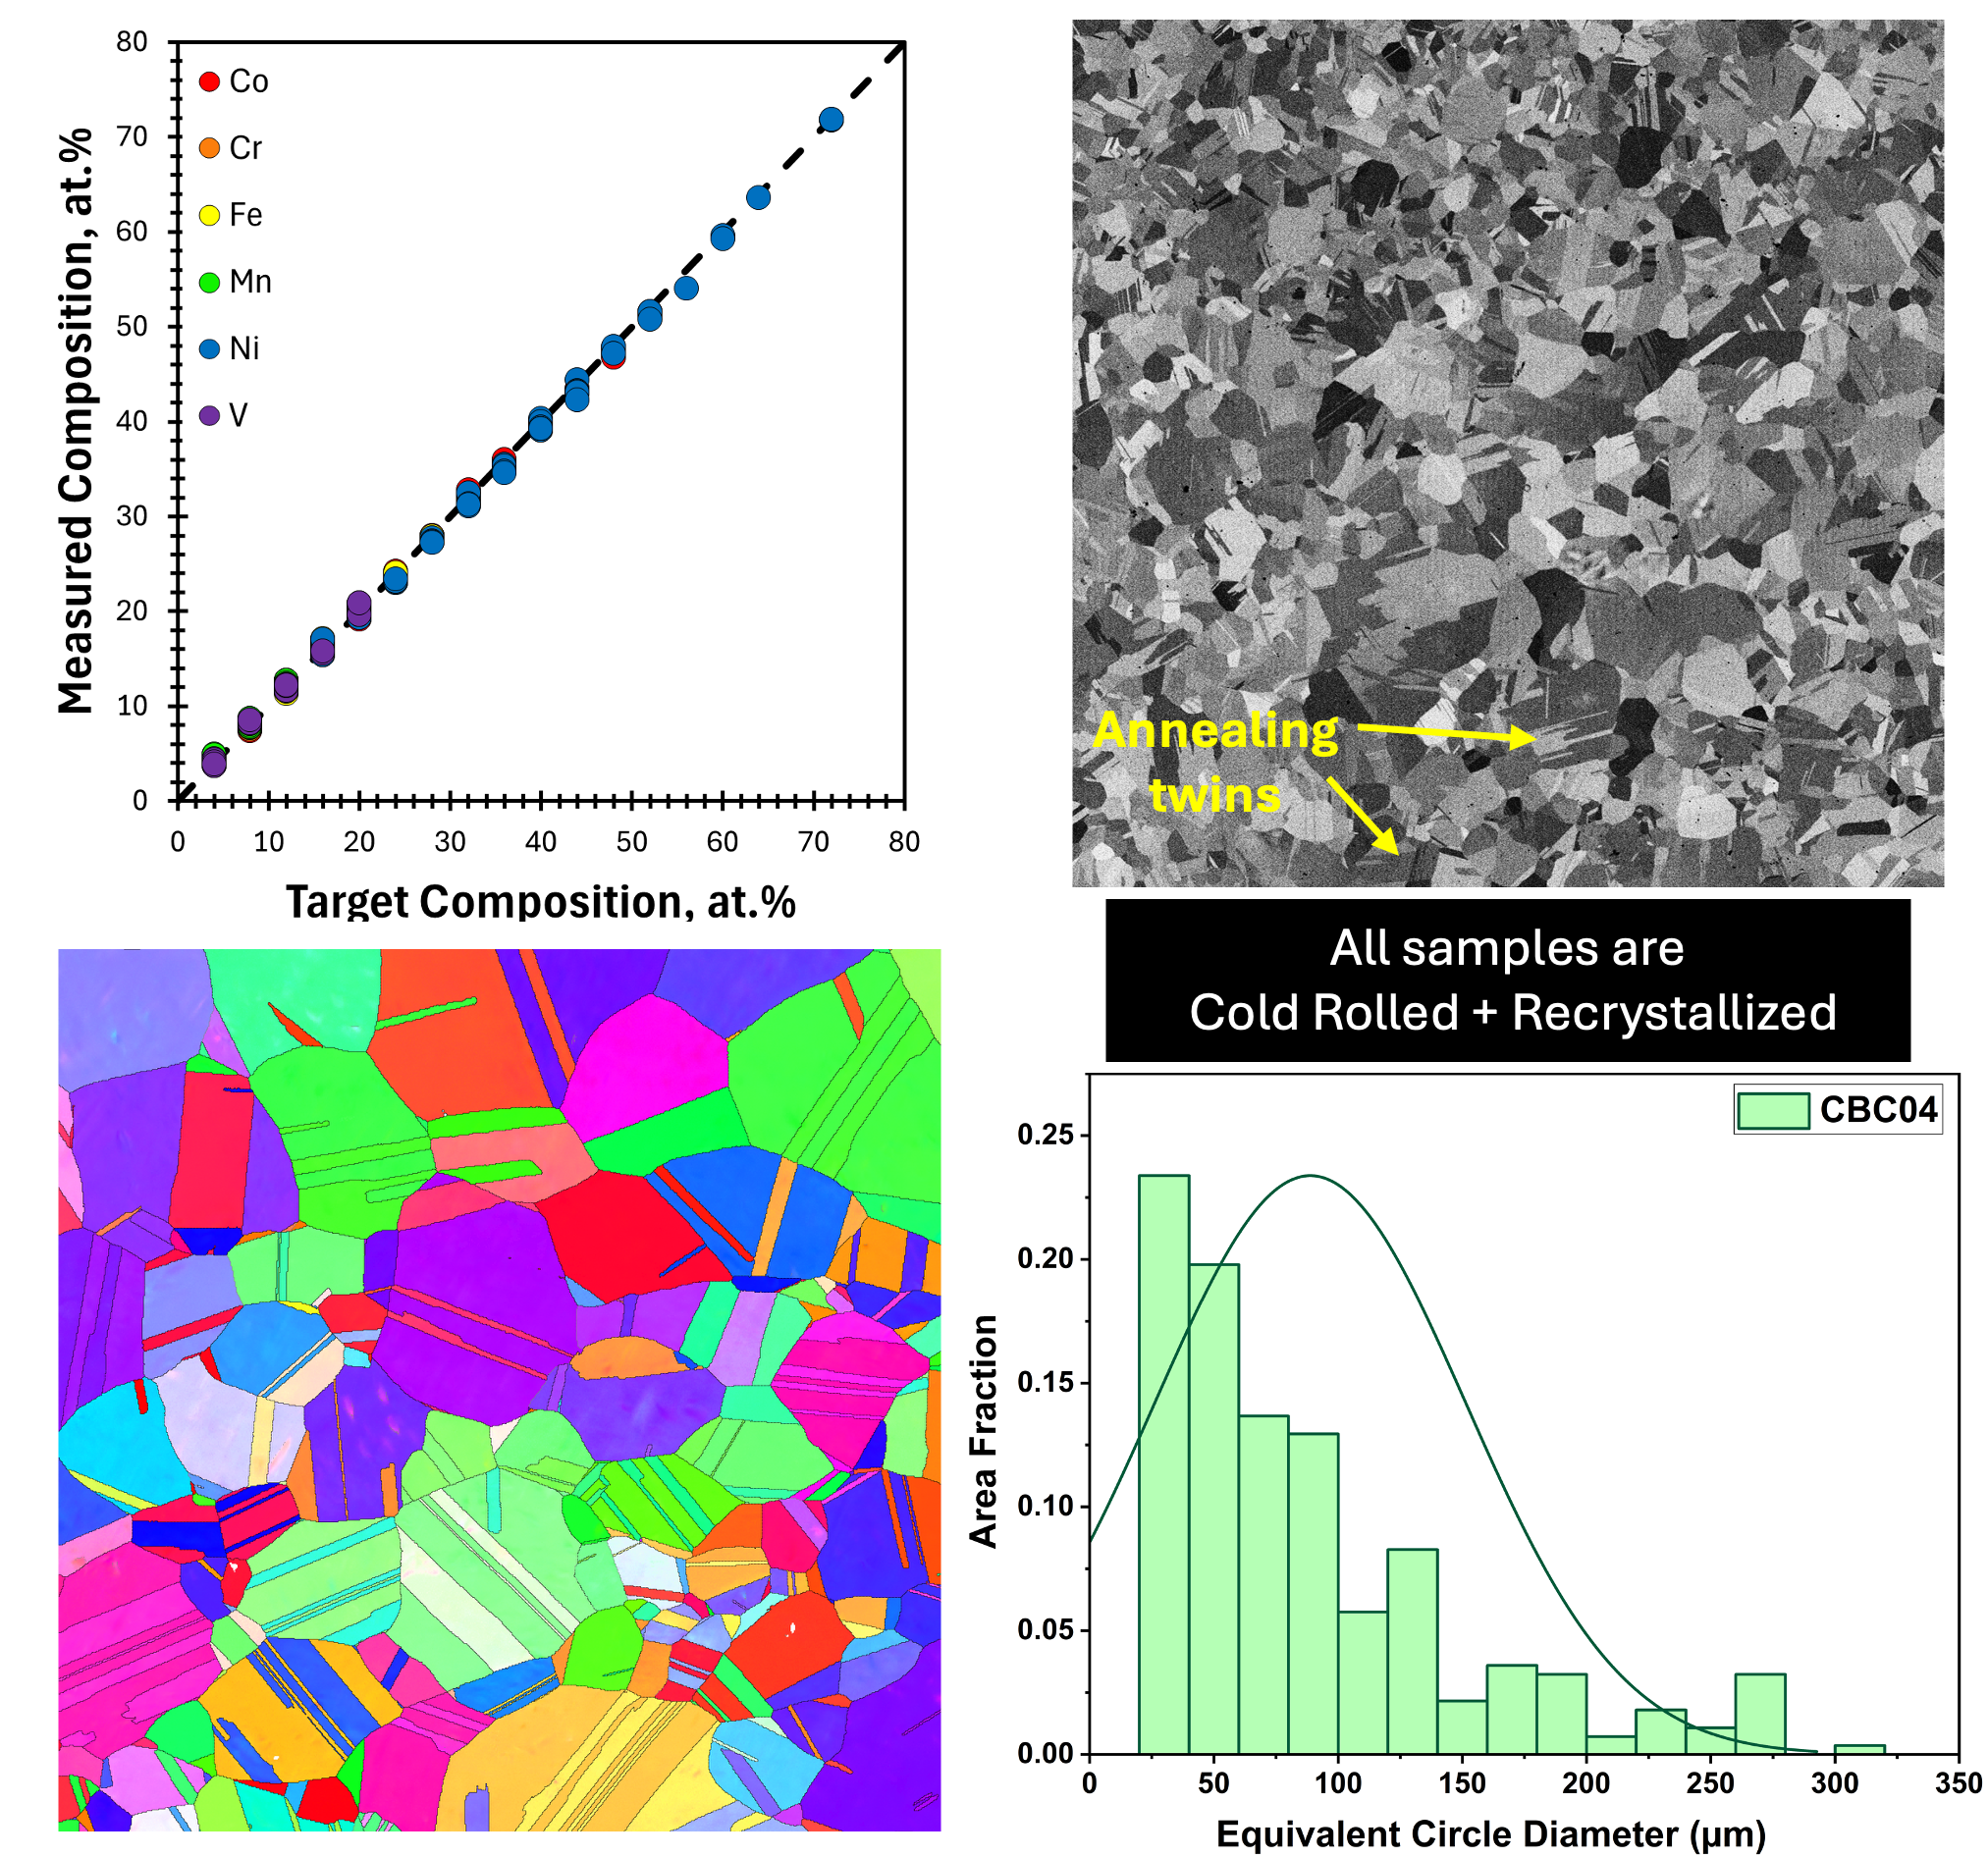
\includegraphics[width=0.85\textwidth]{composition_microstructure.png}
  \caption{Representative synthesis verification for the microstructure-aware campaign: measured (EDS) versus target composition, BSE micrograph and EBSD IPF map of a representative recrystallized alloy (CBC04), and its equivalent-circle-diameter grain-size distribution, whose right-skewed shape motivates tabulating the within-alloy grain-size standard deviation $\text{SD}_\text{grain}$ for every entry.}
  \label{fig:synthesis_verification}
\end{figure}

\begin{figure}[htb]
  \centering
  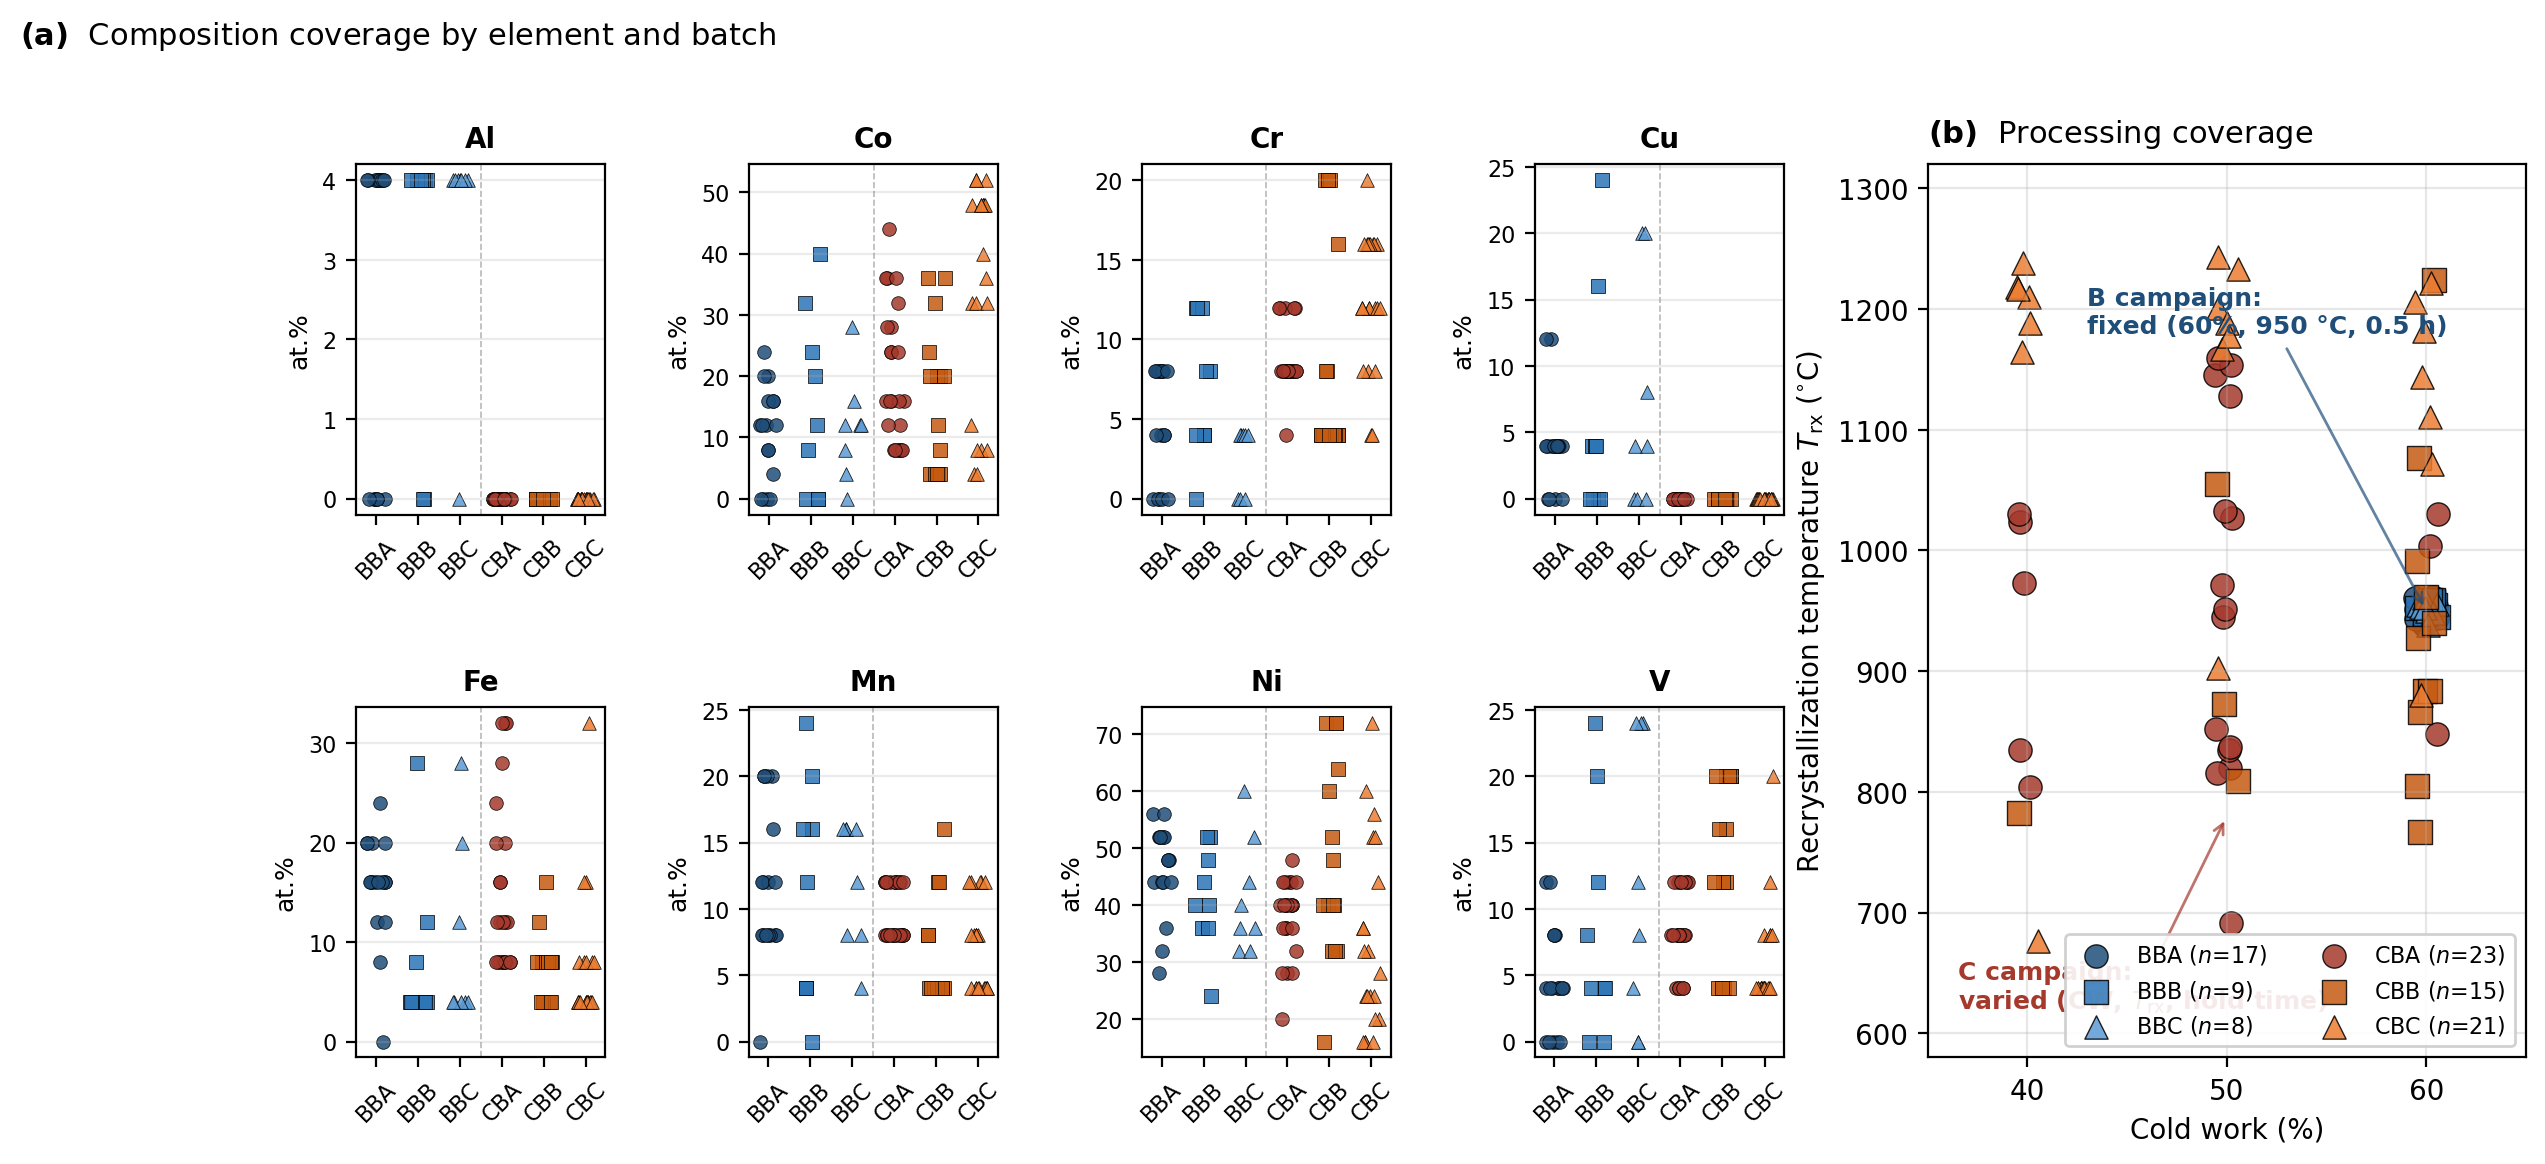
\includegraphics[width=\textwidth]{fig_provenance.png}
  \caption{Provenance of the alloys: (a)~per-element composition coverage across the six BO batches; (b)~processing-parameter coverage. The B campaign collapses to a single processing point; the C campaign fans out across a $3 \times {\sim}10$ grid.}
  \label{fig:provenance}
\end{figure}

\subsection{Property distributions and correlations}

Figure~\ref{fig:property_distributions} shows property distributions stacked by batch.
Yield strength spans 152--544~\si{MPa} (mean $269 \pm 82$), Vickers hardness 58--228 ($133 \pm 33$), and grain size 15--212~\si{\micro\meter} ($58 \pm 43$); the 65--82~\si{\micro\meter} gap in the grain-size histogram reflects the discrete C-campaign processing grid and the B-campaign's single recipe, not a bimodality in grain growth.
Figure~\ref{fig:tensile_curves} shows the underlying true stress--strain curves for the C-campaign alloys.
The top correlates with yield strength are $d^{-1/2}$ ($r = 0.66$), V content ($r = 0.51$), and the VLC misfit parameter $\Phi_\text{VLC}$ ($r = 0.45$); several descriptors are highly mutually correlated (e.g., $\delta$ and $\Phi_\text{VLC}$, $r > 0.9$), motivating regularized and tree-based methods (Fig.~\ref{fig:corr_matrix}).
Residual scatter around the grain-only Hall--Petch fit is strongly correlated with composition, particularly V: V-containing alloys show systematically higher yield strengths at comparable grain sizes, consistent with V's large atomic-size mismatch (134~pm vs.\ $\bar{r} \approx 127$~pm).

\begin{figure}[htb]
  \centering
  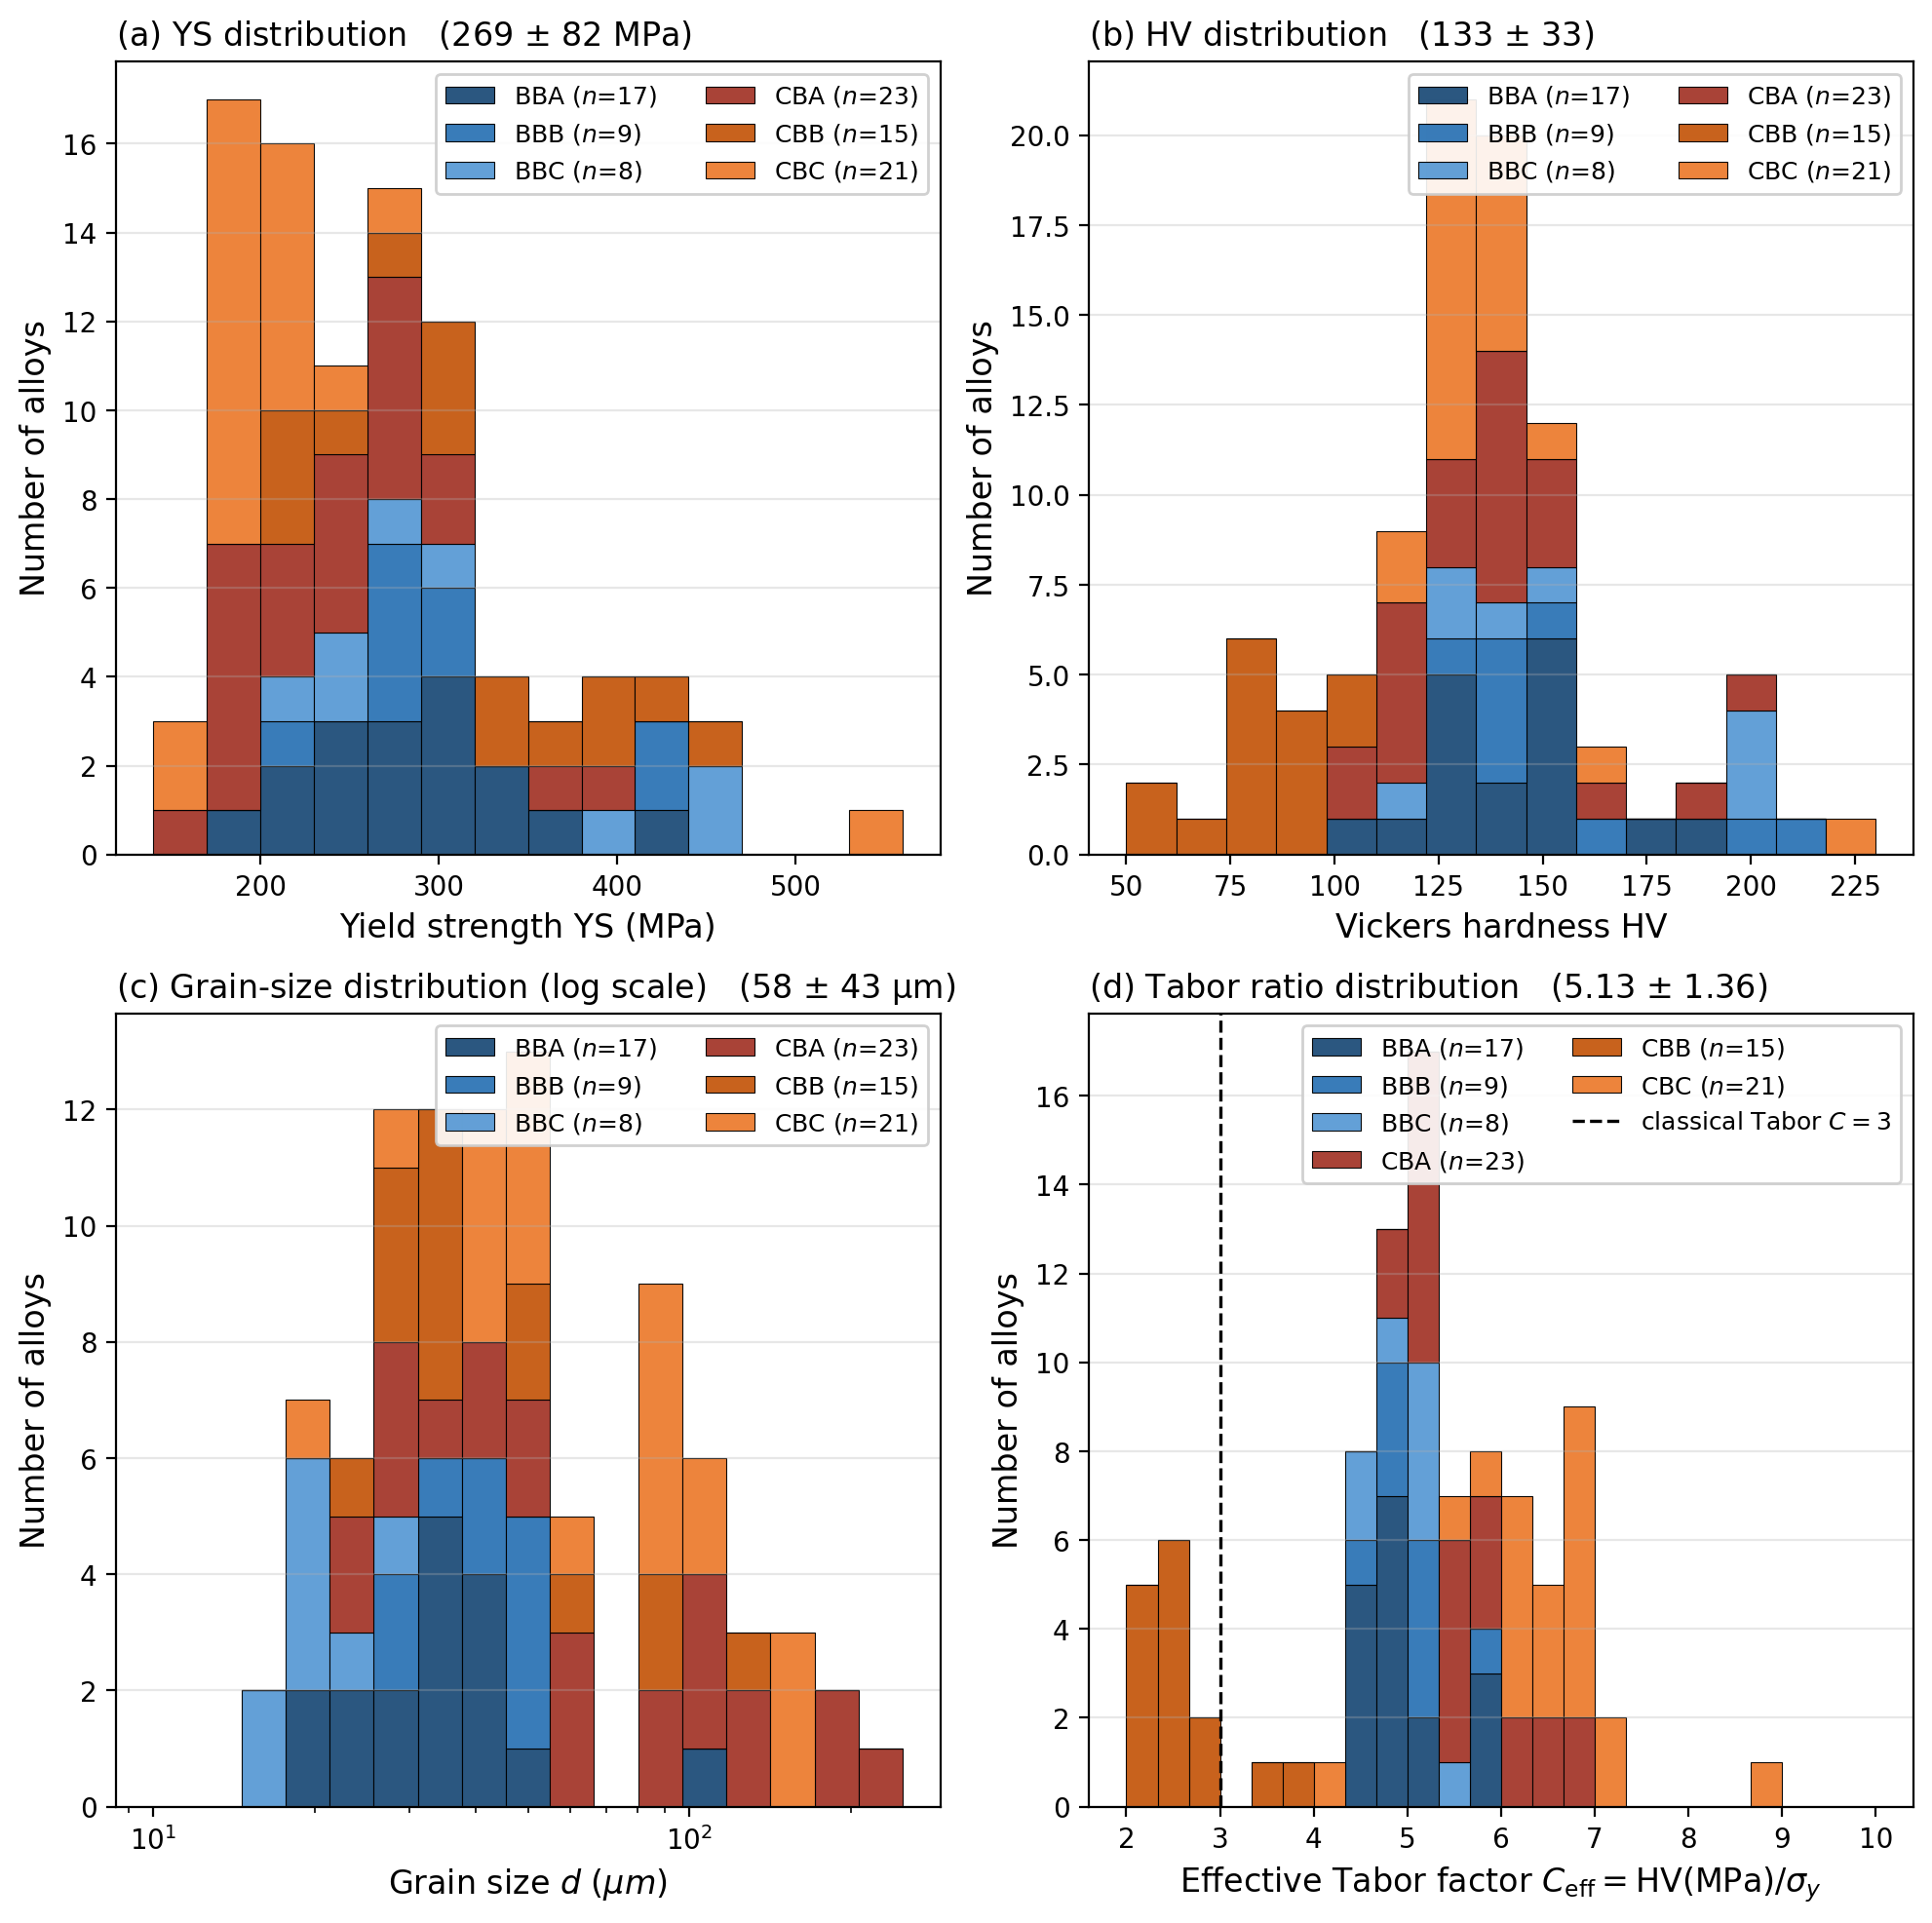
\includegraphics[width=0.7\textwidth]{fig_property_histograms.png}
  \caption{Property distributions across the dataset, stacked by BO batch: (a)~yield strength, (b)~Vickers hardness, (c)~grain size (log axis), (d)~effective Tabor factor $C_\text{eff} = \text{HV(MPa)}/\sigma_y$ ($5.13 \pm 1.36$; dashed line marks the classical $C = 3$).}
  \label{fig:property_distributions}
\end{figure}

\begin{figure}[htb]
  \centering
  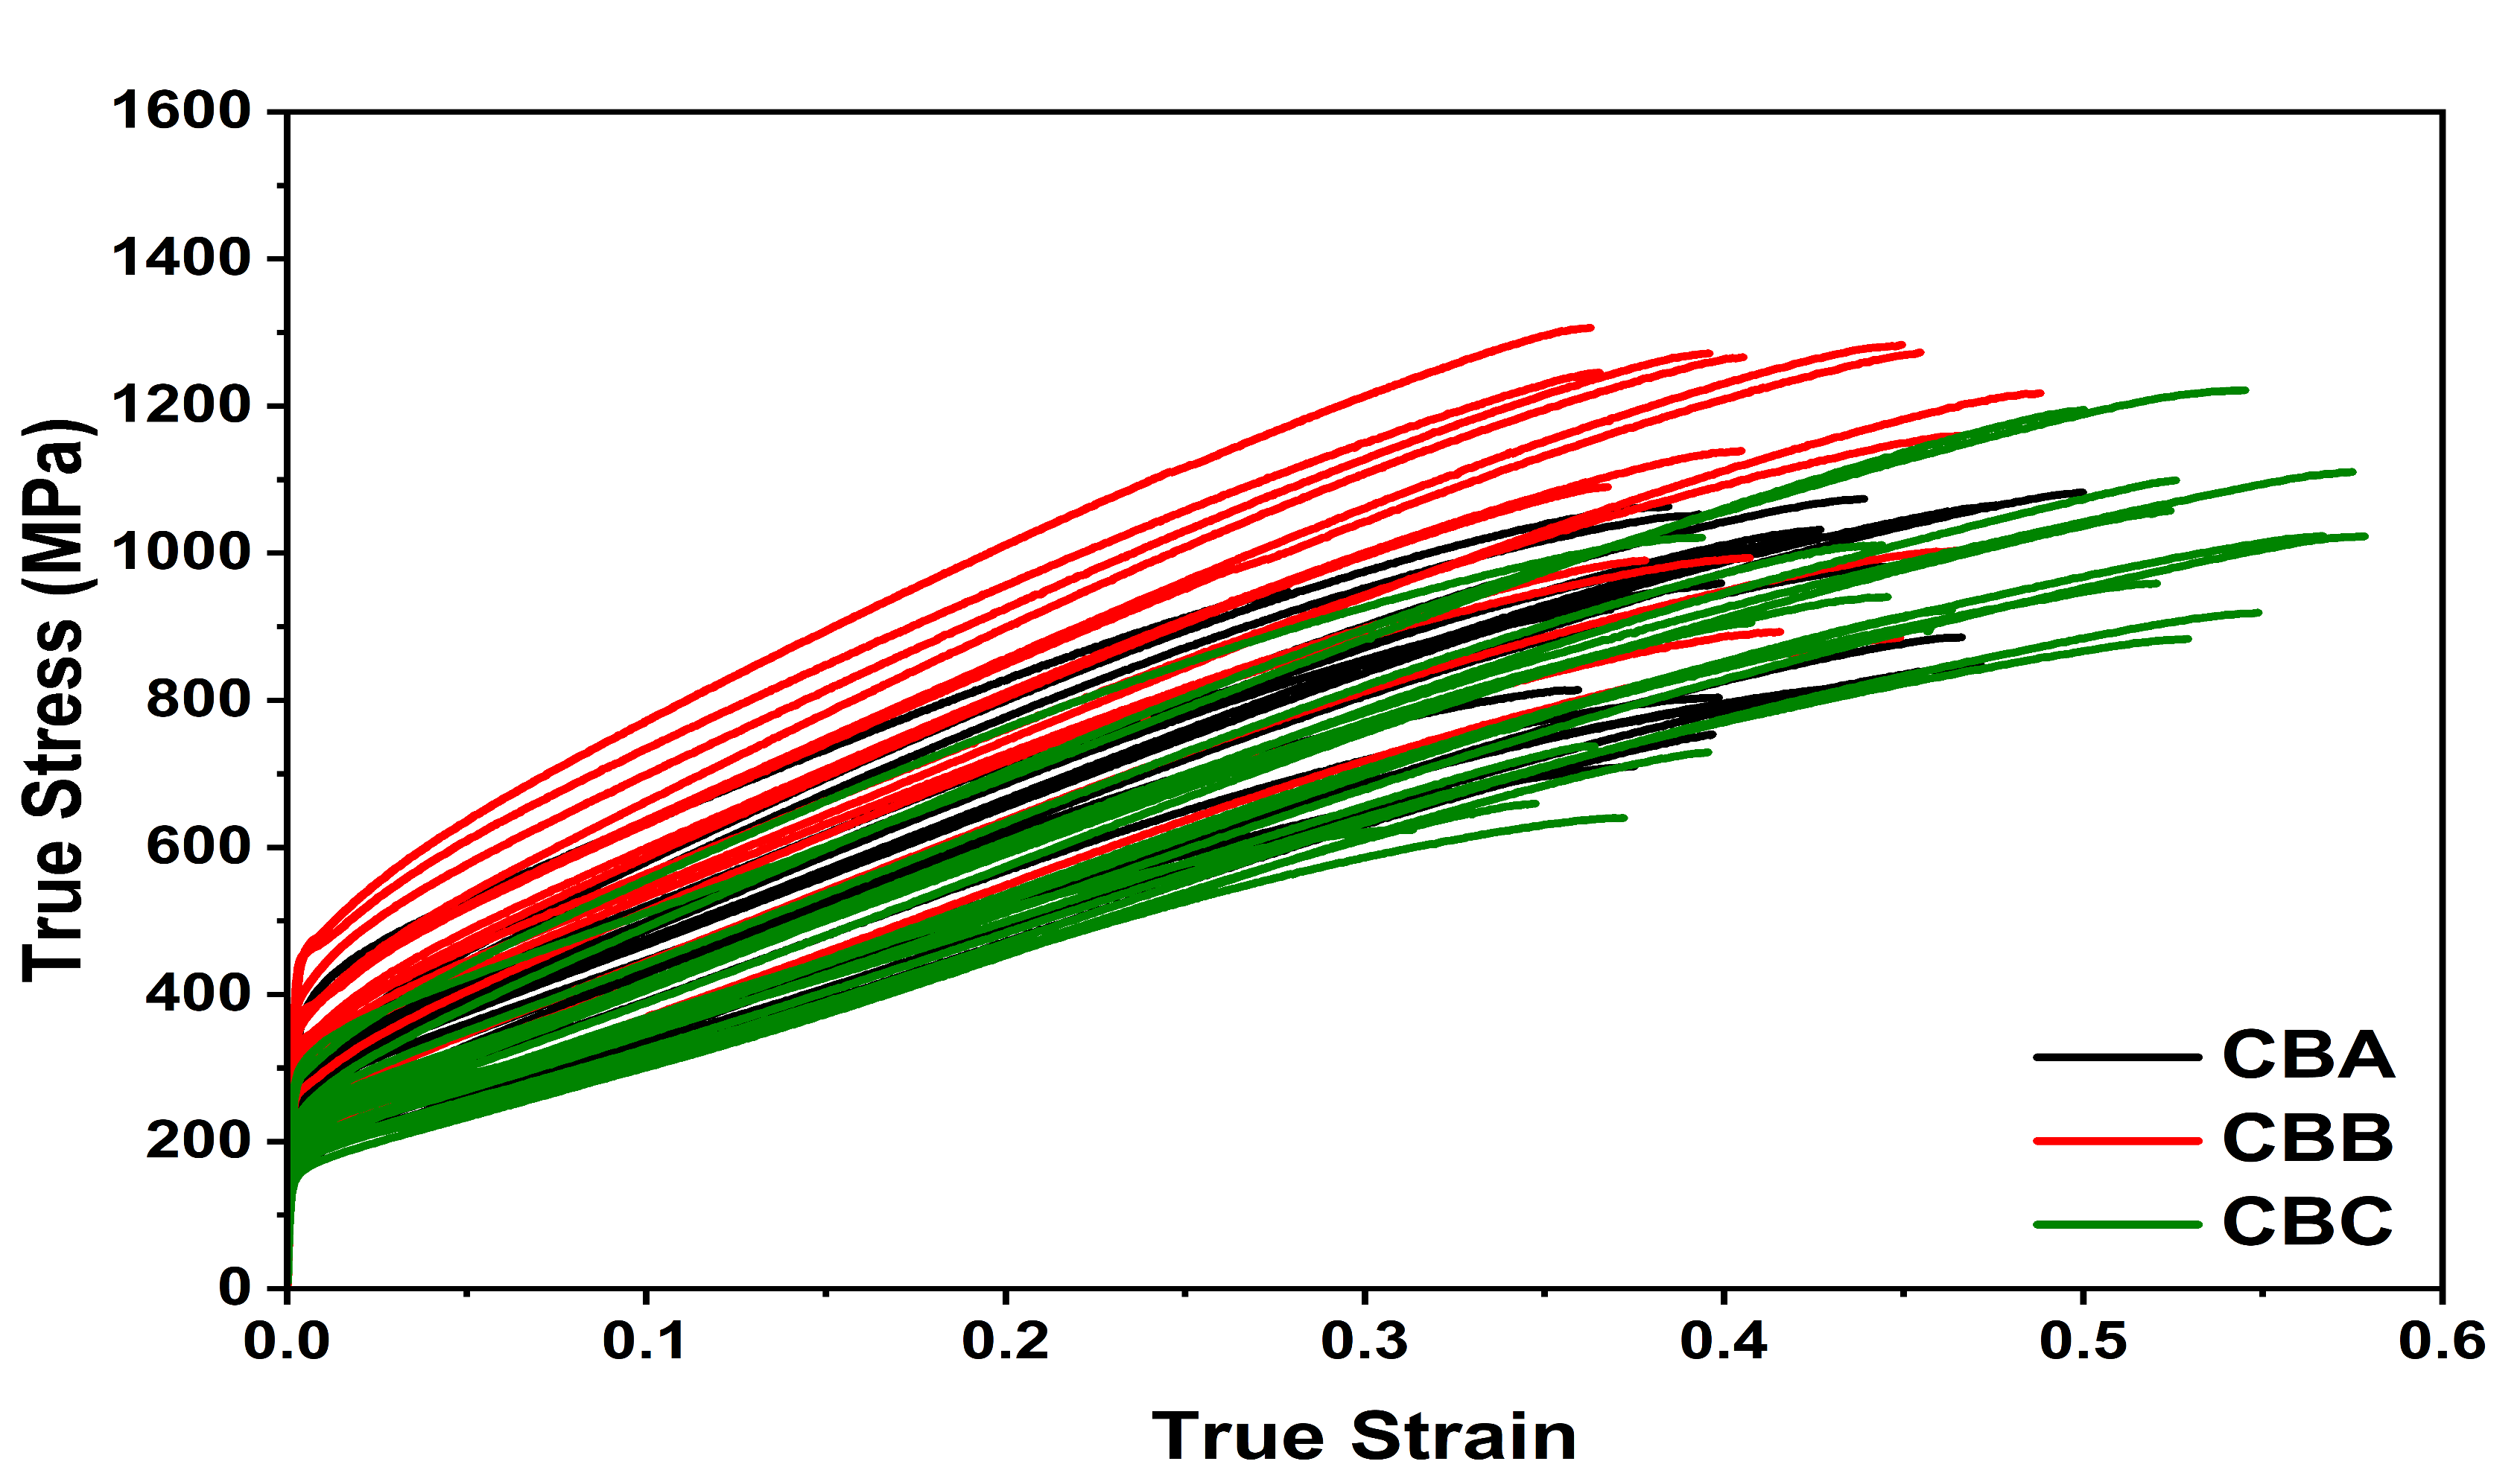
\includegraphics[width=0.7\textwidth]{tensile_tests.png}
  \caption{True stress--strain curves for all C-campaign alloys at $5\times10^{-4}$~s$^{-1}$. The 0.2\% offset yield strengths extracted from these curves are the YS values used throughout the study.}
  \label{fig:tensile_curves}
\end{figure}

\begin{figure}[htb]
  \centering
  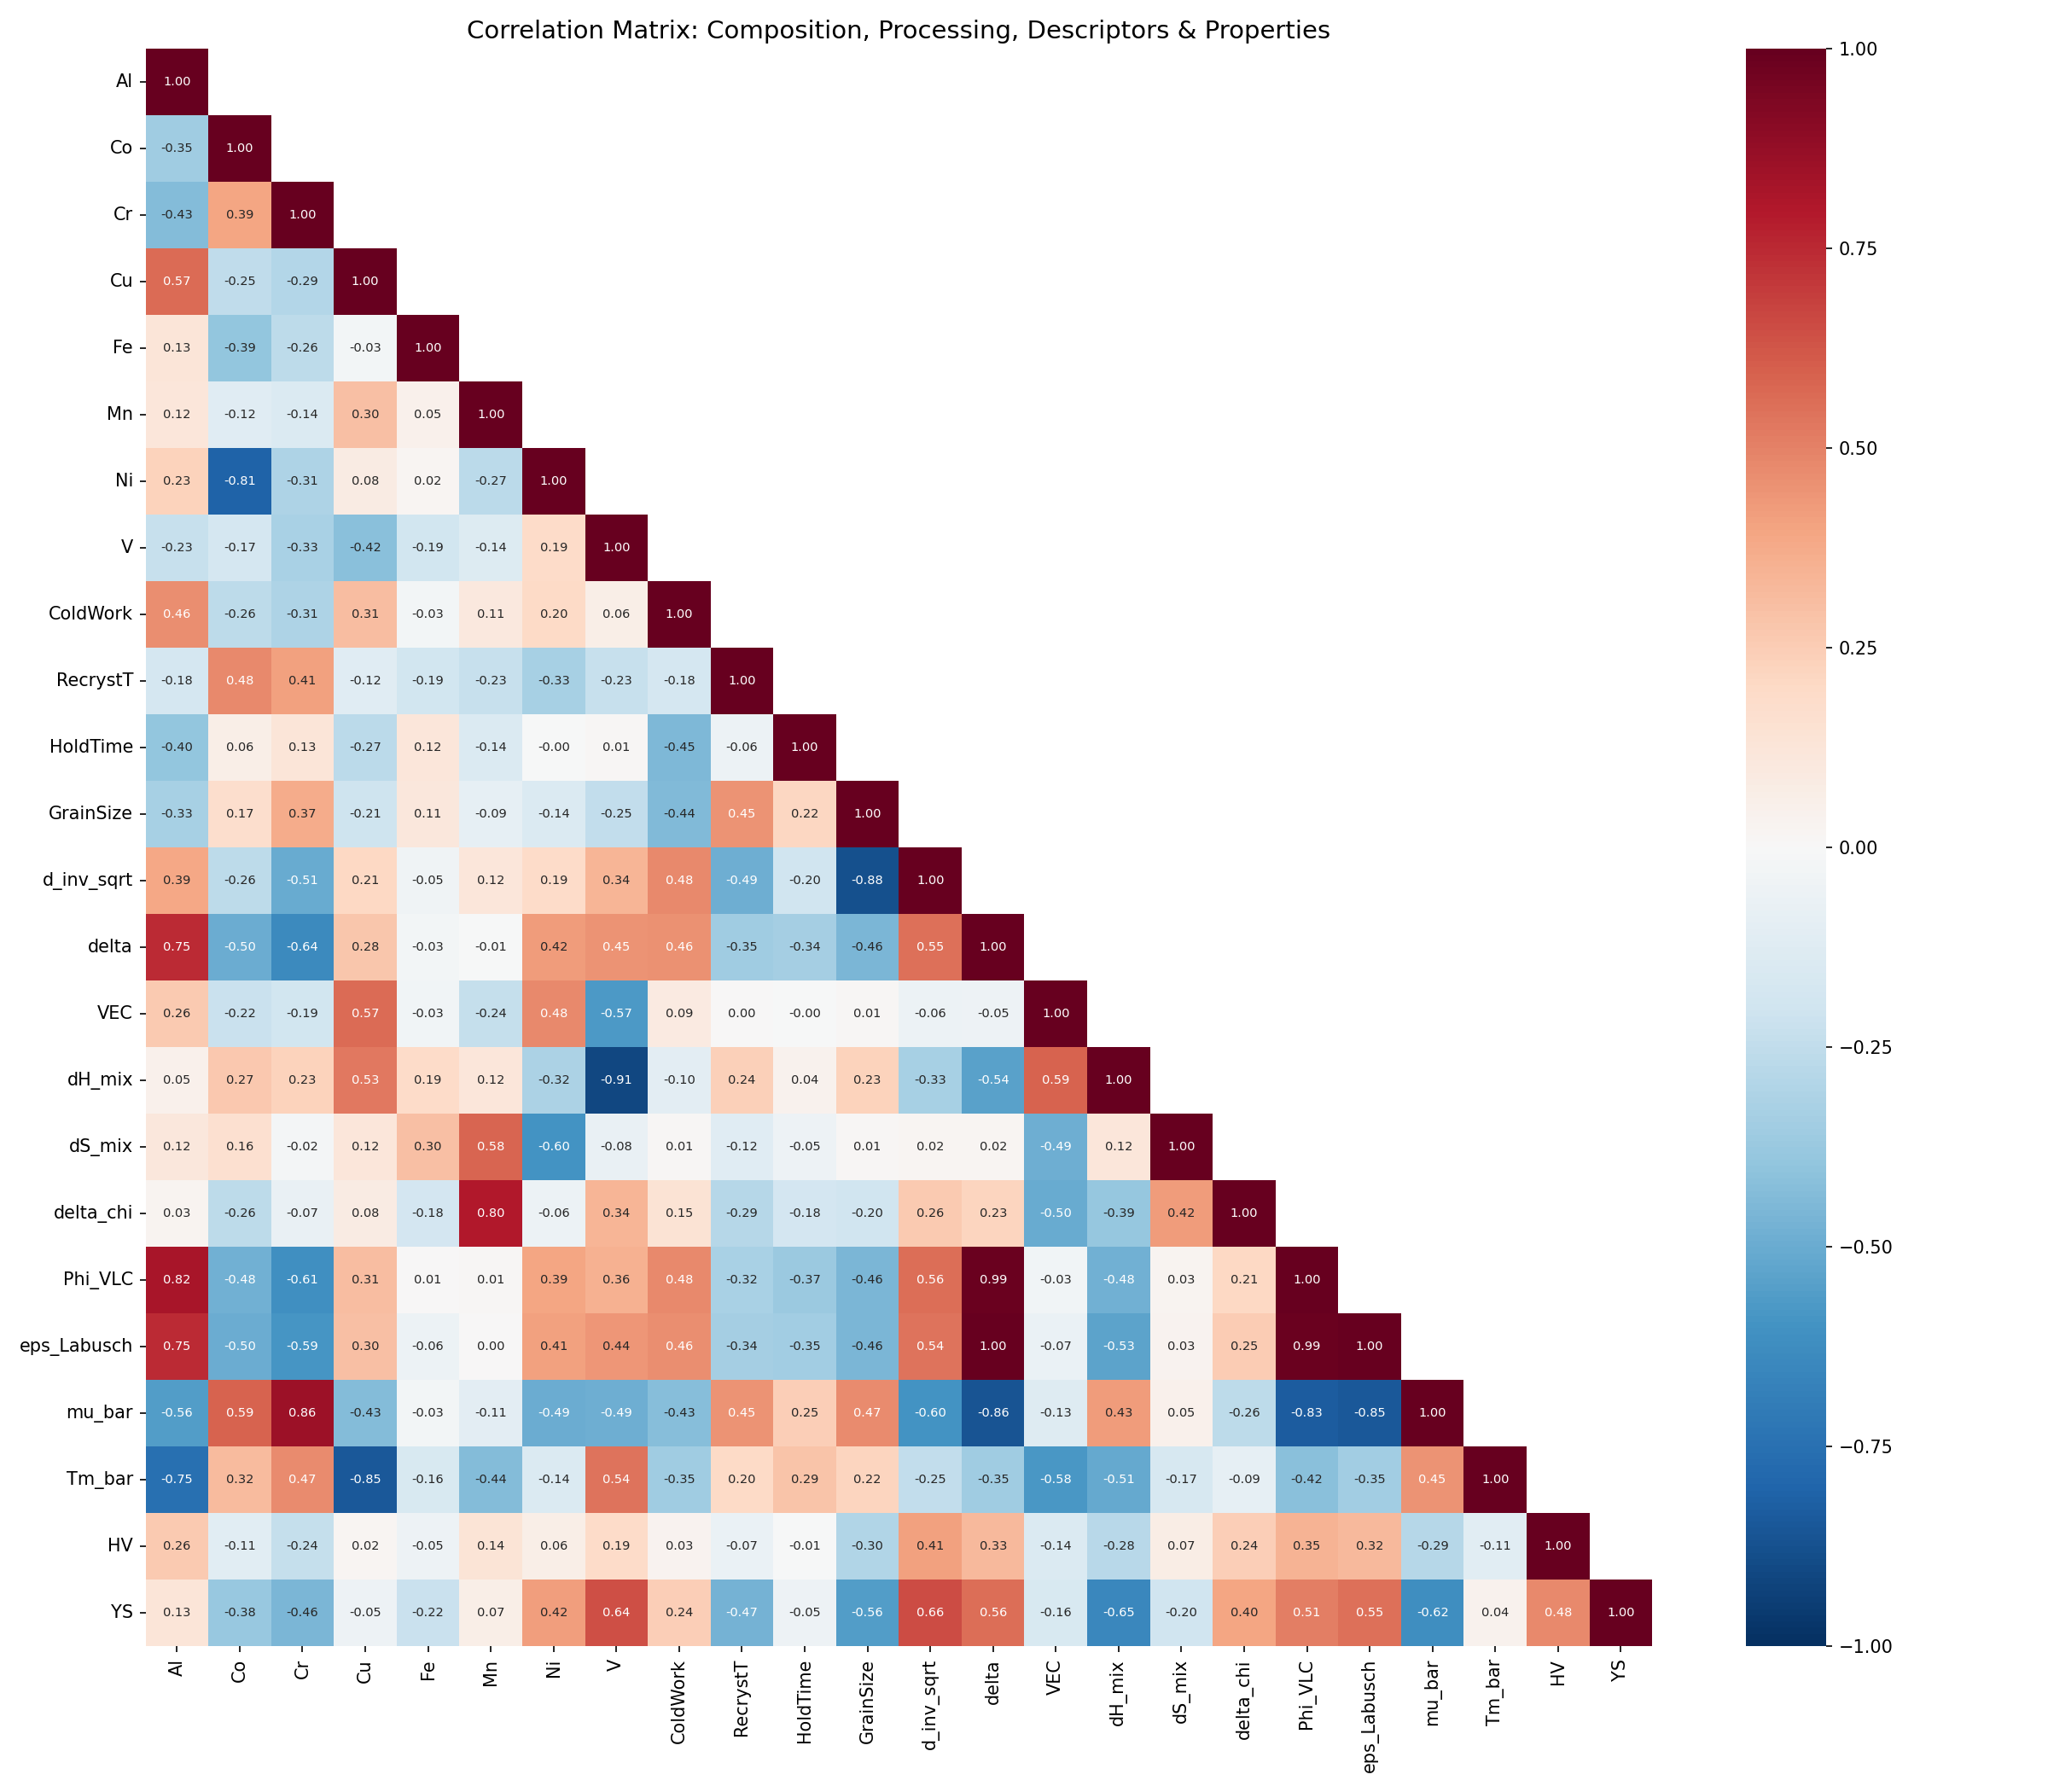
\includegraphics[width=0.75\textwidth]{fig02_correlation_matrix.png}
  \caption{Pearson correlation matrix for composition, processing, and descriptor features.}
  \label{fig:corr_matrix}
\end{figure}

% ============================================================
\section{Pre-modeling diagnostics}
\label{si:premodel}

Before fitting predictive models we examine three questions that bear on everything downstream: (i)~does grain size vary independently of composition? (ii)~how much compositional ground do the six BO batches share? (iii)~what is the highest predictive accuracy any model could plausibly reach?

\emph{Identifiability of the $\sigma_0$/$k_\text{HP}$ partition.}
Cr-rich alloys tend to recrystallize with smaller grains ($r(d, c_\text{Cr}) = +0.38$, $p = 2\times10^{-4}$) and Al-rich alloys with coarser ones ($r = -0.32$).
A multivariate regression of $d^{-1/2}$ on the eight elemental fractions explains 40\% of its variance, rising to 54\% with the three processing variables added.
The remaining ${\sim}46\%$ is independent of chemistry and processing, which makes the $\sigma_0$/$k_\text{HP}$ split identifiable rather than confounded.
Within the 64-feature interaction pool used by the legacy tree models the apparent variance-inflation factor of $d^{-1/2}$ rises to 16.8, but this is artifactual---that pool contains element$\times d^{-1/2}$ cross-terms and other functions of $d^{-1/2}$ by construction; against the physically independent features the inflation is VIF $\approx 1.7$--$2.2$.

\emph{Batch coverage.}
Six principal components are needed to capture 95\% of the compositional variance.
In the dominant PC1--PC2 plane, the average fraction of one batch's compositions falling inside another's convex hull is 0.21 (Fig.~\ref{fig:premodel_pca}), with coverage of the held-out batch by the remaining five ranging from 0.29 (CBC, an isolated V-rich, Cu-free region) to 0.87 (CBA).
An aggregate LOBO $R^2$ therefore averages over qualitatively different held-out tasks---genuine extrapolation in some folds and near-interpolation in others; the per-batch breakdown is given in Section~\ref{si:diagnostics}.

\emph{Noise-limited ceiling.}
Nine of the 81 unique compositions were synthesized more than once; the within-group YS scatter sets the bar for a composition-only predictor at $R^2 \approx 0.86$.
Each alloy was tensile-tested multiple times, and the within-alloy standard deviation (rms $= 15.3$~\si{MPa} over the 80 alloys with replicate tests) sets the noise-limited ceiling for any model using composition and grain size at $R^2 \approx 0.97$.
The best in-sample model of this work (PySR accuracy, LOO $R^2 = 0.765$) reaches roughly 79\% of that ceiling; roughly a fifth of the explainable variance remains unaccounted for by any model tested.

\begin{figure}[htb]
  \centering
  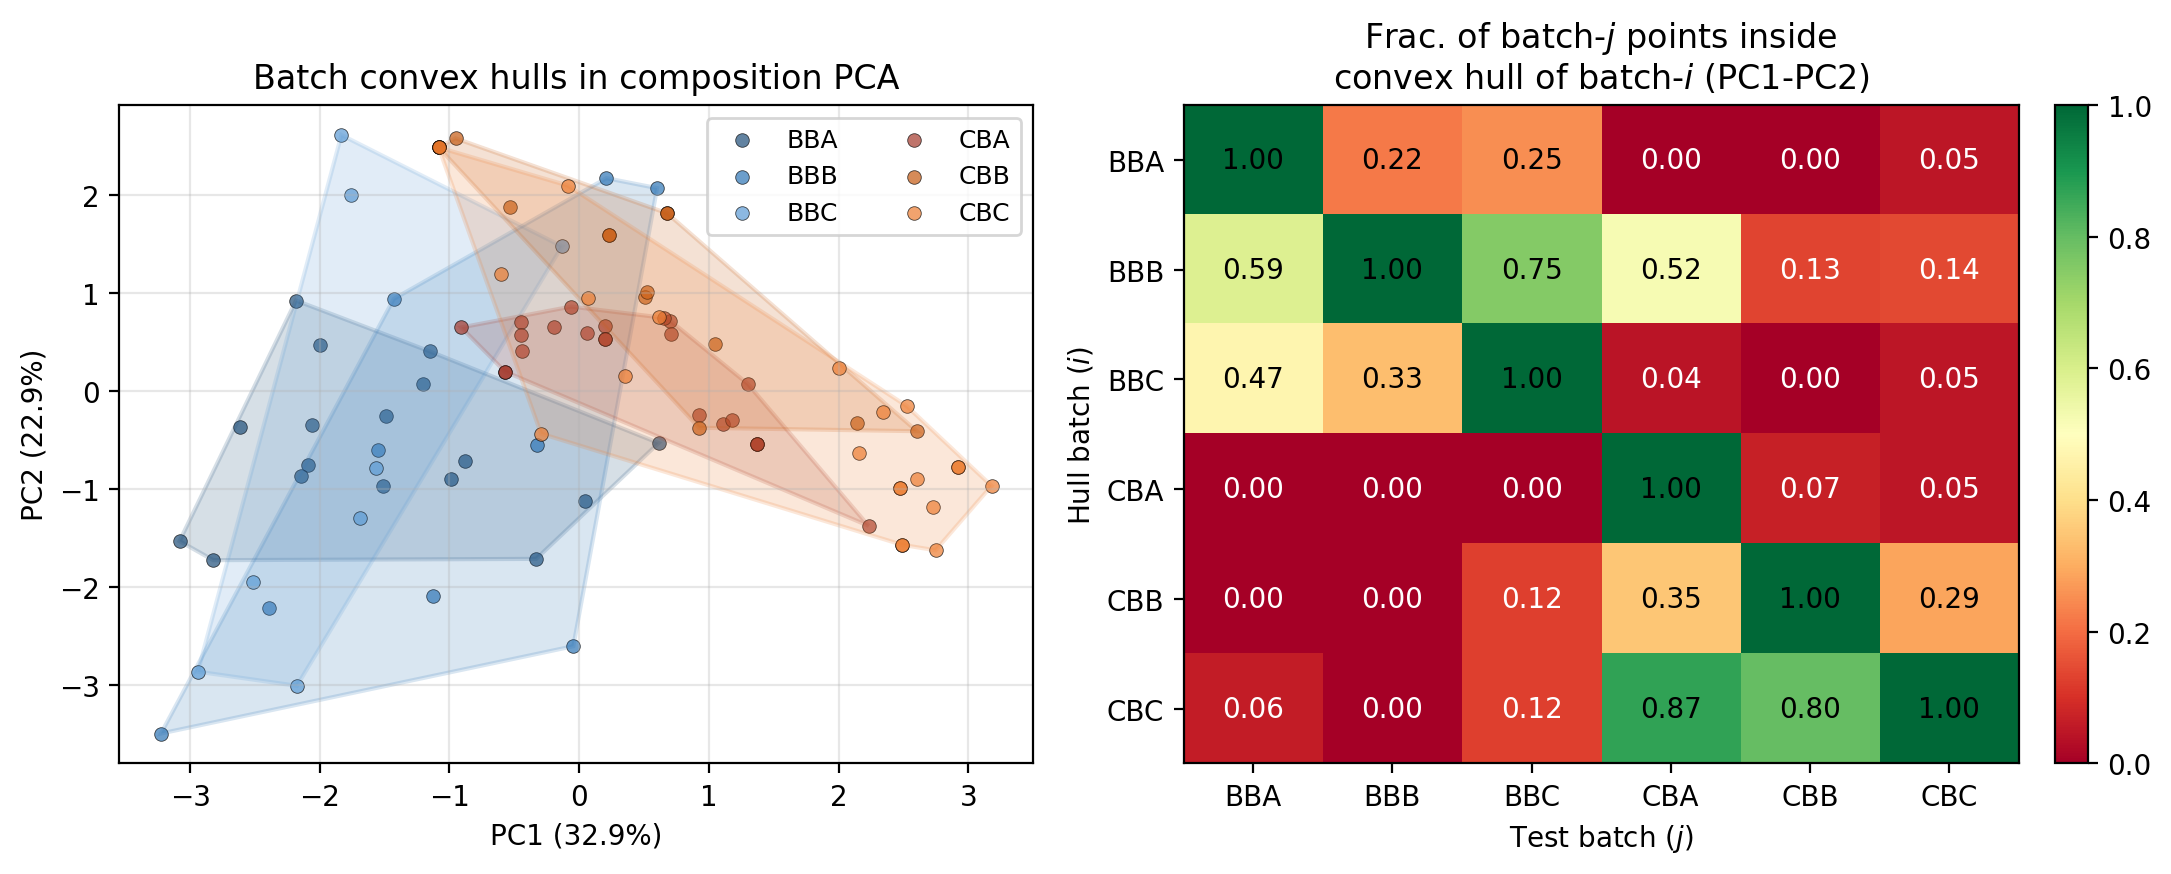
\includegraphics[width=\textwidth]{fig_premodel_hulls_heatmap.png}
  \caption{Batch coverage in composition space (PC1--PC2 of the eight elemental fractions). \textbf{(Left)}~Convex hulls of each BO batch. \textbf{(Right)}~Pairwise hull-overlap matrix; the mean off-diagonal overlap is 0.21, with marked asymmetry (CBC and BBB isolated at 0.29 and 0.33; CBA reachable at 0.87).}
  \label{fig:premodel_pca}
\end{figure}

% ============================================================
\section{Solid-solution strengthening models: formulations and benchmarks}
\label{si:sss}

\subsection{Varvenne--Leyson--Curtin (VLC)}

Following Varvenne et al.~\cite{Varvenne2016,Varvenne2017}, the zero-temperature critical resolved shear stress for a random FCC solid solution is
\begin{equation}
\tau_{y0} = 0.051\,\alpha^{-1/3}\,\bar{\mu}\,\Bigl[\tfrac{1+\bar{\nu}}{1-\bar{\nu}}\Bigr]^{4/3}\,f_1(w_c)\,\Bigl(\sum_i c_i\,\Delta V_i^2\,\big/\,b^6\Bigr)^{2/3},
\label{eq:vlc}
\end{equation}
where $\alpha = 0.123$, $\Delta V_i = V_i - \bar{V}$, $b$ is the Burgers vector, and $f_1(w_c) = 0.35$. The polycrystalline yield stress at temperature $T$ is
\begin{equation}
\sigma_\text{VLC}(T) = M\,\tau_{y0}\,\left[1 - (k_B T / \Delta E_b)^{2/3}\right],
\label{eq:vlc_T}
\end{equation}
with Taylor factor $M = 3.06$~\cite{Dieter1986} and activation barrier
\begin{equation}
\Delta E_b = 0.274\,\alpha^{1/3}\,\bar{\mu}\,b^3\,\Bigl[\tfrac{1+\bar{\nu}}{1-\bar{\nu}}\Bigr]^{2/3}\,f_2(w_c)\,\Bigl(\sum_i c_i\,\Delta V_i^2\,\big/\,b^6\Bigr)^{1/3},
\label{eq:vlc_eb}
\end{equation}
with $f_2(w_c) = 5.70$ and $b = (4\bar{V})^{1/3}/\sqrt{2}$.
For the Ni--Co--Fe--Cr--Mn family the atomic volumes are Varvenne's binary-solid-solution-derived values (Ni: 10.94, Co: 11.12, Fe: 12.09, Cr: 12.27, Mn: 12.60~\AA$^3$); for Al, Cu, and V we use pure-element FCC volumes from tabulated lattice parameters, with the V value extrapolated since pure V is BCC.
Two implementation choices distinguish our computation from Varvenne's published benchmark predictions: rule-of-mixtures elastic constants in place of measured alloy values (a ${\sim}10\%$ upward bias for the Ni--Co--Fe--Cr--Mn family, more for Invar-type compositions), and neglect of the local-environment fluctuation term, which Varvenne also neglects.

\subsection{Labusch (weighted-average HEA extension)}

Following Labusch~\cite{Labusch1970}, the SSS contribution scales as $\sigma \propto \bar{\mu}\,\varepsilon^{4/3}\,c^{2/3}$; our HEA extension is
\begin{equation}
\sigma_\text{Labusch} = \bar{\mu}\,\varepsilon_L^{4/3}\,c_\text{eff}^{2/3}, \quad
\varepsilon_L = \sqrt{\sum_i c_i \left(\delta_{\mu,i}^2 + \alpha_L^2\,\delta_{r,i}^2\right)},
\label{eq:labusch}
\end{equation}
with $\alpha_L = 16$ and $c_\text{eff} = 1/n_\text{comp}$. The classical prefactor (of order $1/Z$ with $Z \approx 60$--$180$) is absorbed into the model.

\subsection{Toda-Caraballo--Rivera-D\'{i}az-del-Castillo}

For an HEA with $n$ active elements at fractions $X_i$~\cite{TodaCaraballo2015},
\begin{equation}
\sigma_\text{TC} = M\,\Bigl(\sum_i B_i^{3/2}\,X_i\Bigr)^{2/3},
\quad
B_i = 3\,\bar{\mu}\,\varepsilon_i^{4/3}\,Z,
\quad
\varepsilon_i = \sqrt{\eta'^2_i + \alpha^2\,\delta_i^2},
\label{eq:tc}
\end{equation}
with damped modulus misfit $\eta'_i = \eta_i / (1 + 0.5\,|\eta_i|)$, $\eta_i = 2(\mu_i - \bar{\mu})/(\mu_i + \bar{\mu})$, Vegard's-law size misfit $\delta_i$, $\alpha = 16$, and $Z = 1/180$ following Labusch's original derivation.
Toda-Caraballo and Rivera-D\'{i}az-del-Castillo do not state a numerical $Z$; their figures use per-pair $B_i$ values fitted to binary-alloy data, which absorb unmodeled effects. Lacking those per-pair values for our eight elements, we fall back on the theoretical $Z$, which makes our implementation structurally faithful but systematically overpredictive by factors of 2--5 without calibration.

\subsection{Cantor-anchored benchmark}

We calibrate the free numerical constants of Labusch and TC once, so that each reproduces $\sigma_\text{SSS}(\text{CoCrFeMnNi}) = 125$~\si{MPa}~\cite{Otto2013}, and hold them fixed: $K_\text{Lab} = 0.027$ implies $Z_\text{Lab} = 1/113$ (within Labusch's range) and $Z_\text{TC} = 1/642$ (outside it). VLC remains parameter-free. The Otto $k_\text{HP} = 494$~MPa$\cdot\mu$m$^{1/2}$ subtracts the grain-size contribution from experiment, giving the target $\sigma_{0,\text{exp}} = \sigma_y - 494\,d^{-1/2}$.
Table~\ref{tab:sss_benchmark} reports alloy-level literature benchmarks, Table~\ref{tab:sss} the 93-alloy panel results, and Fig.~\ref{fig:sss} the parity plot.
Across the panel, calibrated Labusch is the only model with positive raw $R^2$ ($+0.14$) and near-unit magnitude ratio (1.07); TC overshoots by 42\% ($R^2 = -3.18$) and VLC by 78\% ($R^2 = -6.92$). Rank correlations cluster narrowly ($\rho = 0.49$--$0.55$).
As standalone LOO predictors all three fall below Hall--Petch alone (0.406): Labusch 0.274, TC 0.091, VLC 0.030.
In Ridge regressions alongside $d^{-1/2}$, only calibrated Labusch improves the baseline (LOO $R^2 = 0.469$); VLC and TC each reduce it.
With composition fractions present, appending any SSS prediction changes LOO $R^2$ by $\leq 0.002$ and all partial correlations fall below $|r| = 0.10$.

\begin{table}[htb]
\centering
\caption{Benchmark against literature FCC HEAs (Cantor-anchored calibration).}
\label{tab:sss_benchmark}
\small
\begin{tabular}{lcccc}
\toprule
Alloy & $\sigma_\text{VLC}$ & $\sigma_\text{Lab}$ & $\sigma_\text{TC}$ & $\sigma_0$ exp.\ (\si{MPa}) \\
\midrule
NiCoCr~\cite{Yoshida2017}        & 233 & 233 &  135 & 218 \\
NiCoFeCr (Wu 2014)               & 222 & 160 &  146 & 100 \\
CoCrFeMnNi~\cite{Otto2013}       & 243 & 125 &  125 & 125 \\
CoCrFeNiAl (Tung 2007)           & 996 & 645 & 1004 & 800 \\
AlCoCrCuFeNi (Tung 2007)         & 873 & 493 &  854 & 750 \\
\bottomrule
\end{tabular}
\end{table}

\begin{table}[htb]
\centering
\caption{SSS predictions vs.\ the HP-corrected friction stress on the 93-alloy panel. $+$HP columns show Ridge LOO performance of $\sigma_y = a\,\sigma_\text{SSS} + b\,d^{-1/2} + c$.}
\label{tab:sss}
\small
\begin{tabular}{lcccccc}
\toprule
SSS Model & Mean (\si{MPa}) & Ratio & $R^2$ & $\rho$ & $+$HP LOO $R^2$ & RMSE \\
\midrule
VLC (300~K)     & 342 & 1.78 & $-6.92$ & 0.53 & 0.396 & 63.1 \\
Labusch (cal)   & 206 & 1.07 & $+0.14$ & 0.55 & 0.469 & 59.1 \\
TC (cal)        & 274 & 1.42 & $-3.18$ & 0.49 & 0.399 & 62.9 \\
\midrule
HP only         & --- & --- & --- & --- & 0.406 & 62.5 \\
$\sigma_{0,\text{exp}}$ & 193 & 1.0 & --- & --- & --- & --- \\
\bottomrule
\end{tabular}
\end{table}

\begin{figure}[htb]
  \centering
  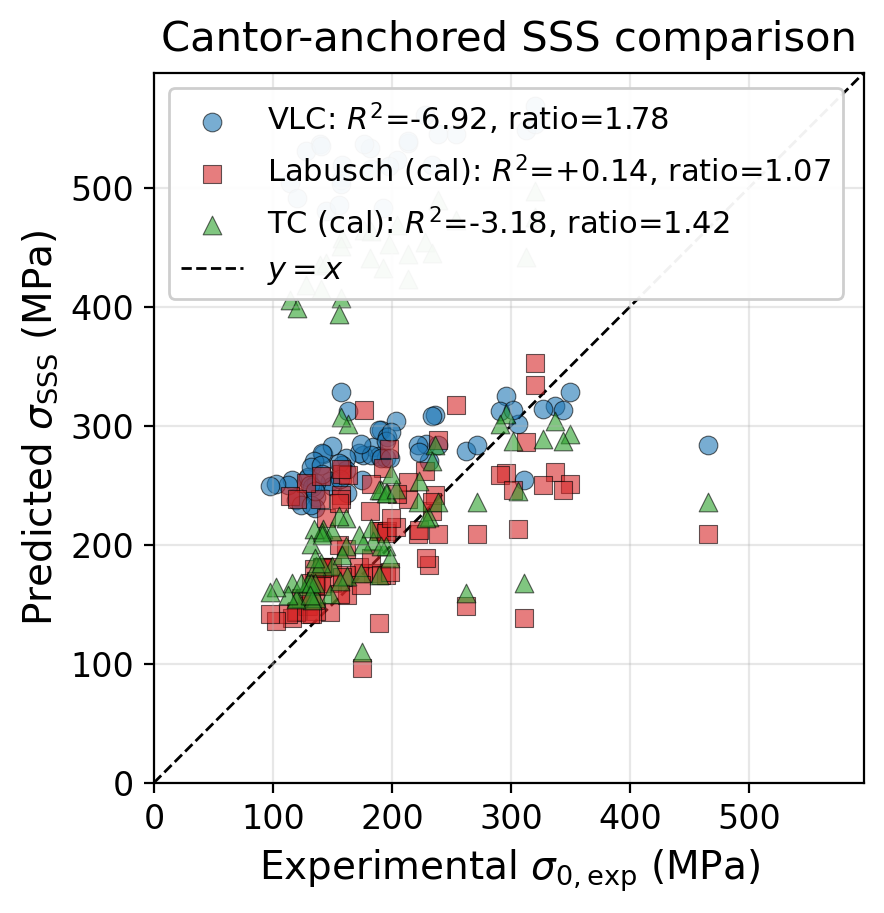
\includegraphics[width=0.6\textwidth]{fig_sss_parity.png}
  \caption{Parity plot of the three SSS predictions vs.\ the Hall--Petch-corrected experimental friction stress.}
  \label{fig:sss}
\end{figure}

The roots of the failure are both methodological and fundamental: Vegard's-law volumes linearly extrapolate lattice parameters from pure-element FCC structures that V and Al do not adopt, producing sign-dependent errors (underprediction near equimolar, 4--5$\times$ overprediction for V/Al-rich) that no rescaling can fix.
VLC with DFT-derived misfit volumes achieves quantitative accuracy for equimolar FCC HEAs~\cite{Varvenne2016,Moitzi2022}, and with experimentally measured misfits and elastic constants it rationalizes nanoindentation hardness across 24 single-phase FCC Co-Cr-Fe-Mn-Ni alloys~\cite{Bracq2019}, so it is the input approximation, not the theory, that fails; physics-based models may retain value for extrapolation where data-driven models lose validity~\cite{Khatamsaz2023}.

% ============================================================
\section{Grain-size scaling laws: full results}
\label{si:scaling}

Table~\ref{tab:scaling} reports the frequentist comparison of the nine scaling laws for YS, Table~\ref{tab:bayesian_scaling} the Bayesian PSIS-LOO comparison, Table~\ref{tab:within_alloy_scaling} the within-replicate fits, and Table~\ref{tab:hv_scaling} the HV comparison.
The Hall--Petch posterior yields $\sigma_0 = 92 \pm 22$~\si{MPa} and (grain-only) $k_\text{HP} = 1149 \pm 140$~MPa$\cdot\mu$m$^{1/2}$; this inflated slope arises because the global grain-only regression conflates composition effects with the HP slope (V-rich alloys are systematically stronger and finer-grained, $r(V, d) = -0.24$).
Allowing $\sigma_0$ to depend on composition (M3) collapses the slope to $k_\text{HP} = 766$~MPa$\cdot\mu$m$^{1/2}$, within the FCC-HEA literature range.
The free-exponent posterior is $n = 0.53 \pm 0.16$ (94\% HDI $[0.22, 0.82]$, $P(0.4 < n < 0.6) = 0.43$); the 94\% credible band of the model-averaged prediction ($\pm{\sim}30$~\si{MPa}) is far narrower than the data scatter ($\pm{\sim}150$~\si{MPa}), making the dominance of composition-driven variance directly visible (Figs.~\ref{fig:scaling_fits}--\ref{fig:bayesian_bma}).
The best-leveraged replicate group (Co-Cr-Fe-Mn-Ni-V, $n = 3$, $d = 23$--$188$~\si{\micro\meter}) yields $k_\text{local} = 731$~MPa$\cdot\mu$m$^{1/2}$ with within-group $R^2 = 0.995$, consistent with the global M3 value.

\begin{table}[htb]
\centering
\caption{Comparison of grain-size scaling laws for YS: $\sigma_y = \sigma_0 + k\,f(d)$, ranked by BIC.}
\label{tab:scaling}
\small
\begin{tabular}{lcccccc}
\toprule
Scaling law $f(d)$ & $k$ & Train $R^2$ & LOO $R^2$ & LOO RMSE & BIC & $\Delta$BIC \\
\midrule
$d^{-1/2}$ [Hall--Petch] & 2 & 0.429 & 0.406 & 62.5 & 774.5 & 0.0 \\
$\ln(d)/d$ & 2 & 0.429 & 0.406 & 62.5 & 774.5 & 0.0 \\
$d^{-2/3}$ & 2 & 0.429 & 0.405 & 62.6 & 774.6 & 0.1 \\
$d^{-1/3}$ [Baldwin] & 2 & 0.427 & 0.403 & 62.6 & 774.9 & 0.4 \\
$d^{-1}$ [Dunstan--Bushby] & 2 & 0.419 & 0.395 & 63.1 & 776.1 & 1.6 \\
$\ln(d)$ & 2 & 0.413 & 0.388 & 63.4 & 777.2 & 2.7 \\
$d^{-0.548}$ [Optimized] & 3 & 0.430 & 0.406 & 62.5 & 779.0 & 4.5 \\
$1/\sqrt{d} + 1/d$ [Composite] & 3 & 0.430 & 0.395 & 63.1 & 779.0 & 4.5 \\
$d^{-1} + d^{-2}$ [Taylor] & 3 & 0.429 & 0.387 & 63.5 & 779.1 & 4.6 \\
\bottomrule
\end{tabular}
\end{table}

\begin{table}[htb]
\centering
\caption{Bayesian comparison via PSIS-LOO (YS). Stacking weights optimized for out-of-sample prediction.}
\label{tab:bayesian_scaling}
\small
\begin{tabular}{lcccc}
\toprule
Model & elpd$_\text{loo}$ & $\Delta$LOO & $p_\text{loo}$ & Weight \\
\midrule
Hall--Petch $d^{-1/2}$              & $-518.5$ & 0.0 & 4.2 & 1.000 \\
Composite $d^{-1/2}\!+\!d^{-1}$     & $-518.5$ & 0.1 & 4.2 & 0.000 \\
Critical thickness $\ln(d)/d$       & $-518.5$ & 0.1 & 4.3 & 0.000 \\
Intermediate $d^{-2/3}$              & $-518.7$ & 0.2 & 4.4 & 0.000 \\
Baldwin $d^{-1/3}$                  & $-518.7$ & 0.2 & 4.2 & 0.000 \\
Optimized exponent $d^{-n}$         & $-518.8$ & 0.3 & 4.5 & 0.000 \\
Logarithmic $\ln(d)$                & $-519.7$ & 1.2 & 3.9 & 0.000 \\
Dunstan--Bushby $d^{-1}$            & $-520.3$ & 1.8 & 4.3 & 0.000 \\
\bottomrule
\end{tabular}
\end{table}

\begin{table}[htb]
\centering
\caption{Within-alloy scaling-law fits on the 9 multi-replicate composition groups (21 alloys).}
\label{tab:within_alloy_scaling}
\small
\begin{tabular}{lcc}
\toprule
Scaling law & Pooled within-group $R^2$ & $R^2$ ($n{=}3$ group) \\
\midrule
$d^{-1/2}$ [Hall--Petch]   & 0.778 & 0.995 \\
$d^{-1/3}$ [Baldwin]       & 0.781 & 0.997 \\
$d^{-2/3}$                 & 0.775 & 0.993 \\
$d^{-1}$ [Dunstan--Bushby] & 0.769 & 0.987 \\
$\ln(d)/d$ [crit.\ thick.] & 0.776 & 0.993 \\
$\ln d$                    & 0.786 & 0.999 \\
\bottomrule
\end{tabular}
\end{table}

\begin{table}[htb]
\centering
\caption{Grain-size scaling laws fit to HV, ranked by $\Delta$BIC.}
\label{tab:hv_scaling}
\small
\begin{tabular}{lcccc}
\toprule
Scaling law $f(d)$ & $k$ & Train $R^2$ & LOO $R^2$ & $\Delta$BIC \\
\midrule
$d^{-1.728}$ [Optimized]   & 3 & 0.193 & 0.166 & 0.0 \\
$d^{-1}$ [Dunstan--Bushby] & 2 & 0.185 & 0.154 & 0.9 \\
$d^{-2/3}$                 & 2 & 0.175 & 0.143 & 2.1 \\
$\ln(d)/d$                 & 2 & 0.174 & 0.141 & 2.3 \\
$d^{-1/2}$ [Hall--Petch]   & 2 & 0.169 & 0.136 & 2.8 \\
$d^{-1/3}$ [Baldwin]       & 2 & 0.161 & 0.128 & 3.7 \\
$1/\sqrt{d} + 1/d$         & 3 & 0.192 & 0.151 & 4.7 \\
$\ln(d)$                   & 2 & 0.144 & 0.110 & 5.6 \\
\bottomrule
\end{tabular}
\end{table}

\begin{figure}[htb]
  \centering
  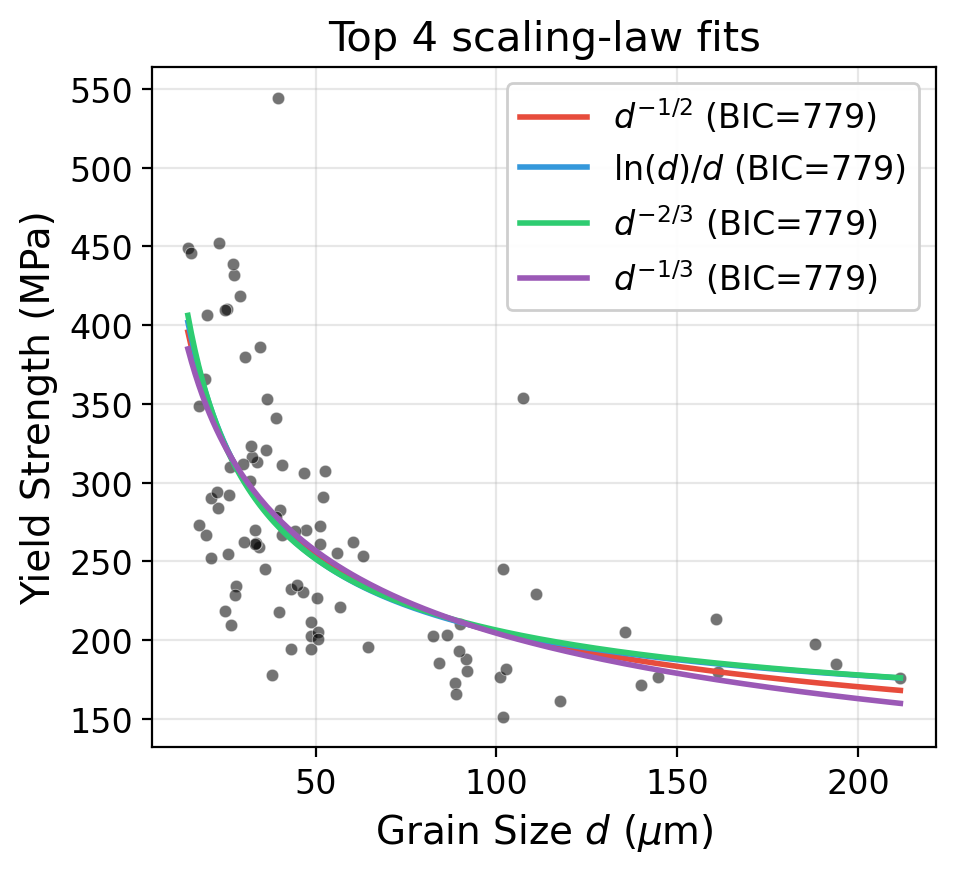
\includegraphics[width=0.55\textwidth]{fig_scaling_fits.png}
  \caption{The top four YS scaling laws overlap visibly across the full $d$ range.}
  \label{fig:scaling_fits}
\end{figure}

\begin{figure}[htb]
  \centering
  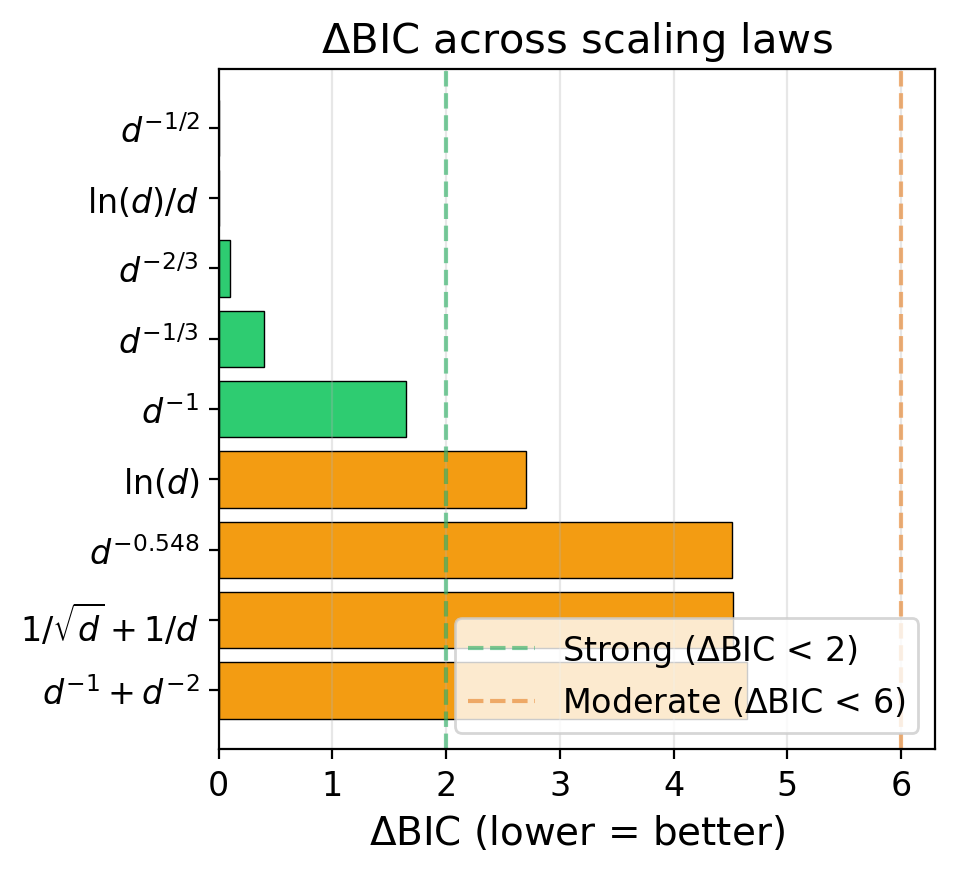
\includegraphics[width=0.55\textwidth]{fig_scaling_deltabic.png}
  \caption{$\Delta$BIC for the nine candidate scaling laws relative to Hall--Petch (YS).}
  \label{fig:scaling_deltabic}
\end{figure}

\begin{figure}[htb]
  \centering
  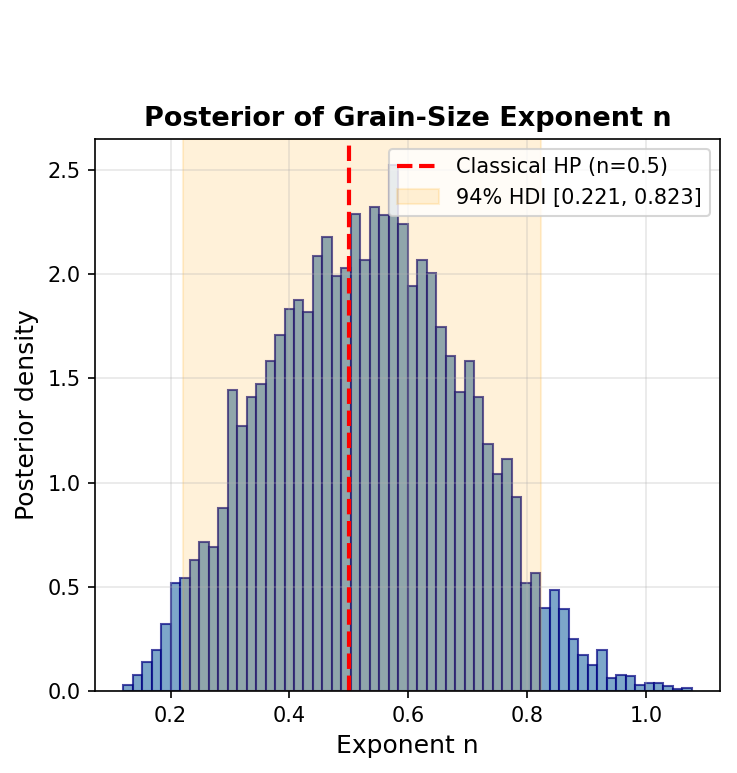
\includegraphics[width=0.55\textwidth]{fig_bayesian_n.png}
  \caption{Marginal posterior of the grain-size exponent in $\sigma_y = \sigma_0 + k\,d^{-n}$; the dashed line marks $n = 0.5$.}
  \label{fig:bayesian_exponent}
\end{figure}

\begin{figure}[htb]
  \centering
  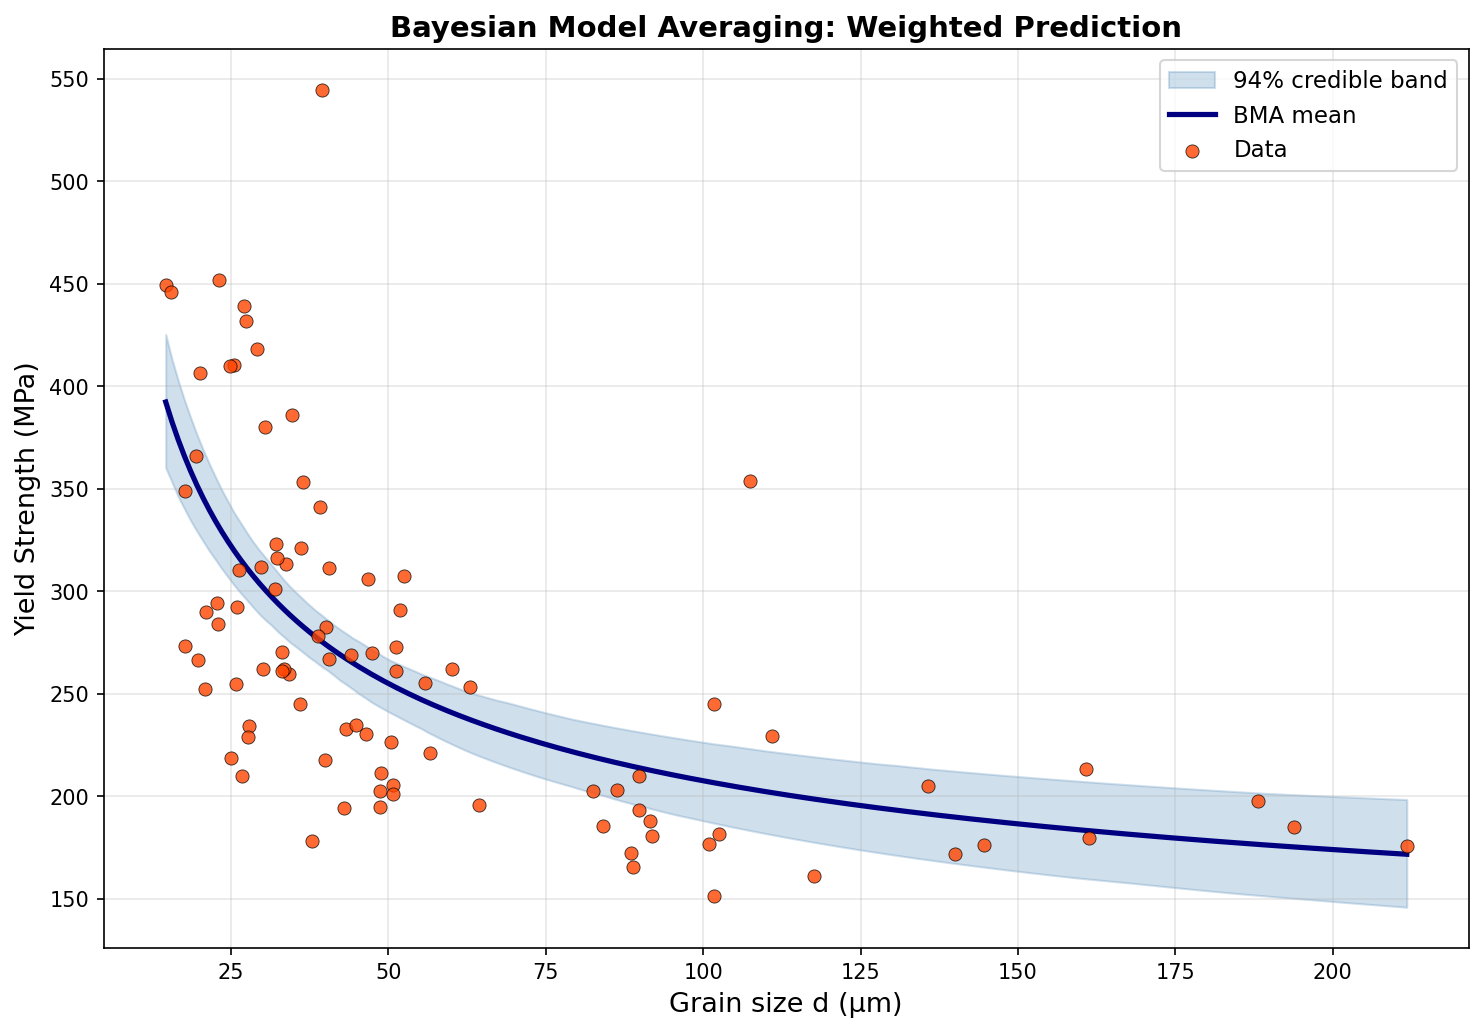
\includegraphics[width=0.55\textwidth]{fig_bayesian_bma.png}
  \caption{Bayesian model-averaged prediction with 94\% credible band versus the observed alloys.}
  \label{fig:bayesian_bma}
\end{figure}

% ============================================================
\section{Legacy 17-model panel, feature sets, and SHAP analysis}
\label{si:mlpanel}

The legacy panel predates the equal-footing protocols of the main text and is retained because it measures the validation failure mode at full strength.
It spans 17 models across six families (linear, kernel, tree, compact boosting, physics-informed, ensemble) on six hierarchical feature sets: CORE (12: element fractions $+$ $d^{-1/2}$ $+$ processing), PHYSICS (27: $+$15 descriptors), PHYSICS\_ALT (33: $+$alternative grain-size features), INTERACTIONS (46: $+$11 cross-terms), INTERACTIONS\_ALT (64: $+$element$\times d^{-1}$ and SSS$\times$grain products), and COMPACT (top-20 by mutual information).
Tuned models used Optuna with 50 Bayesian trials on the full dataset prior to LOO---the optimism this induces is quantified here and eliminated in the ARMOTE-CV and fair-comparison panels of the main text.
Table~\ref{tab:models} shows the ranking.

\begin{table}[htb]
\centering
\caption{Legacy panel ranked by LOO $R^2$ (models with $R^2 < 0$ omitted). INT\_ALT $=$ INTERACTIONS\_ALT.}
\label{tab:models}
\small
\begin{tabular}{llrrrrrr}
\toprule
Model & Features & $n_f$ & LOO $R^2$ & RMSE & LOBO $R^2$ & $k_\text{eff}$ & BIC \\
\midrule
XGBoost & INT\_ALT & 64 & 0.729 & 42.2 & 0.574 & 3749 & 16889 \\
Average Ensemble & meta & 5 & 0.700 & 44.4 & --- & 5 & 728 \\
Stacking (Ridge) & meta & 5 & 0.698 & 44.6 & 0.707 & 6 & 717 \\
Random Forest & INT\_ALT & 64 & 0.675 & 46.3 & 0.623 & 320 & 2046 \\
LightGBM & INT\_ALT & 64 & 0.673 & 46.4 & 0.625 & 320 & 1935 \\
SVR (RBF) & COMPACT & 20 & 0.654 & 47.7 & 0.497 & 83 & 1062 \\
M3: $\sigma_0$(all) & HP\_PHYS & 9 & 0.652 & 47.8 & 0.625 & 10 & 743 \\
XGBoost-compact & COMPACT & 20 & 0.650 & 48.0 & 0.580 & 1484 & 7259 \\
Ridge & PHYS\_ALT & 33 & 0.638 & 48.8 & 0.651 & 34 & 847 \\
ElasticNet & PHYS\_ALT & 33 & 0.637 & 48.9 & 0.648 & 32 & 839 \\
CatBoost & INT\_ALT & 64 & 0.637 & 48.9 & 0.515 & 600 & 2845 \\
\bottomrule
\end{tabular}
\end{table}

Three caveats attach to this panel.
The stacking ensemble's apparent negative LOO--LOBO gap (0.698 vs.\ 0.707) reflects mild leakage: its meta-features are LOO predictions from base models that saw other members of each held-out batch during training.
XGBoost's LOO--LOBO gap of 0.155 indicates that roughly 21\% of its explained variance derives from batch-specific patterns.
BIC comparisons across families are approximate because $k_\text{eff}$ estimation differs (regression parameters vs.\ total leaves vs.\ $n$ for interpolating kernels).

SHAP analysis of the best XGBoost model (Fig.~\ref{fig:shap}) ranks $\Omega$ first, followed by the interaction features Mn$\times d^{-1}$ and V$\times d^{-1}$, alternative grain-size features, and the SSS descriptors.
The dominance of element$\times d^{-1}$ over element$\times d^{-1/2}$ terms is geometric: tree models partition feature space through axis-aligned splits, and the $d^{-1}$ transformation stretches the fine-grained regime where strengthening effects are largest, enabling more informative splits; in linear models the two transformations are near-collinear and interchangeable.
As established in the main text, these interaction features act as flexible proxies for the composition-dependent $\sigma_0$, not as evidence of a composition-dependent slope.

\begin{figure}[htb]
  \centering
  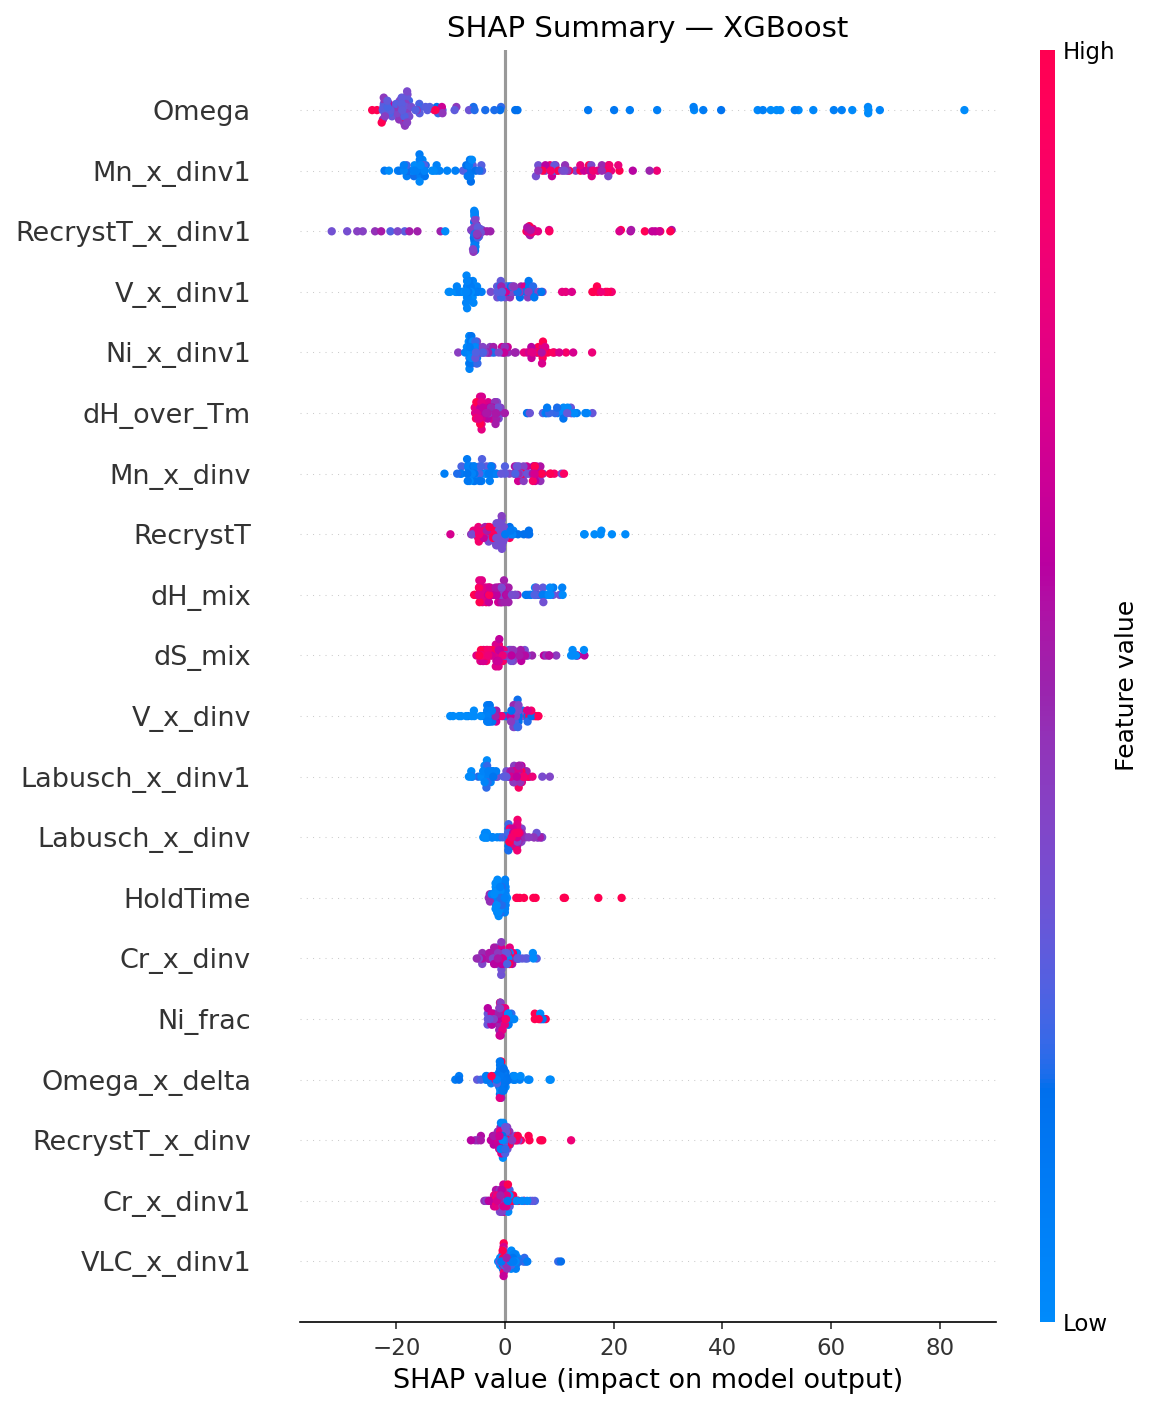
\includegraphics[width=0.6\textwidth]{fig07_shap_summary.png}
  \caption{SHAP summary for the legacy XGBoost model (top 20 features by mean $|\text{SHAP}|$).}
  \label{fig:shap}
\end{figure}

% ============================================================
\section{Symbolic regression: search details and expanded controls}
\label{si:sr}

\subsection{SISSO configuration}
The SISSO input space contains 27 features: Oliynyk-style statistics (mean, variance, delta, range) of atomic radii, shear modulus, electronegativity, and melting point~\cite{Oliynyk2016}; HEA thermodynamic descriptors; the SSS parameters $\Phi_\text{VLC}$, $\varepsilon_L$, $\sigma_\text{TC}$; and $d^{-1/2}$.
Two tiers of algebraic expansion ($+,-,\times,\div$) precede $\ell_0$-regularized selection at dimension $D = 3$ (four effective parameters).
The robust variant was obtained by excluding $\delta_\mu$ from the pool; three independent searches (varying which delta-type features are excluded) converge to the same equation.
In the $\text{SD}_\text{grain}$-augmented runs the pool additionally contains $\text{SD}_\text{grain}$ and the processing variables.

\subsection{Expanded-search controls}
SISSO v2 adds unary operators ($x^2$, $\sqrt{x}$, $x^{-1}$), raises the SIS threshold to 30, adds nine alternative grain-size features ($d^{-\alpha}$ for eight exponents plus $\ln d$), and selects $D \in \{1,\ldots,4\}$ by BIC.
Despite the larger space (36 primary features, 3293 after expansion), SISSO v2 achieves lower LOO $R^2 = 0.604$ and LOBO $R^2 = 0.350$: different folds select different grain-size features, degrading cross-validated performance.
At dimension 1 the best single feature is $d^{-0.45}/\Omega$; higher dimensions prefer $\ln d$---consistent with the BIC-indistinguishable scaling laws of Section~\ref{si:scaling}.
Constraining the search to $d^{-1/2}$ stabilizes model selection across folds and yields superior generalization: in small-sample symbolic regression the right inductive bias outweighs a broader search.
EML universal-operator regression ($\texttt{eml}(x,y) = e^x - \ln y$)~\cite{Odrzywolek2025} reaches only LOO $R^2 = 0.321$ at depth 1 (20 effective parameters) and overfits catastrophically at greater depth.
The recalibrated pure-metal Hall--Petch model of Jiang et al.~\cite{Jiang2022HP} reaches LOO $R^2 = 0.346$, below the grain-only baseline: its rule-of-mixtures descriptors ($\bar{W}$ varies by only $\pm 12\%$, $\bar{\alpha}$ by $\pm 8\%$, $\bar{\gamma}_\text{GB}$ by $\pm 9\%$ across the panel) cannot discriminate alloys within the narrow Ni-rich window, whereas the variance descriptors SISSO selects vary 15--30-fold.

\subsection{PySR grid summary}
Table~\ref{tab:pysr_grid} reports the elbow-selected equations across the full feature $\times$ operator grid with external validation.

\begin{table}[htb]
\centering
\caption{PySR grid (elbow selections) with external validation. Const $=$ fitted constants; Ext $=$ external RMSE (MPa for YS, HV units for HV); Safe $=$ singularity-audit outcome.}
\label{tab:pysr_grid}
\small
\begin{tabular}{llcccccc}
\toprule
Target & Cell & Const & LOO $R^2$ & LOBO $R^2$ & BIC & Ext & Safe \\
\midrule
YS & F1$\cdot$O1 & 1 & 0.019 & $-0.251$ & 818 & 112 & yes \\
YS & F1$\cdot$O2 & 2 & 0.482 & 0.276 & 761 & 168 & yes \\
YS & F1$\cdot$O3 & 1 & 0.399 & 0.205 & 773 & 158 & yes \\
YS & F2$\cdot$O2 & 2 & 0.605 & 0.475 & 737 & 114 & yes \\
YS & F2$\cdot$O3 & 2 & 0.604 & 0.496 & 737 & 108 & yes \\
YS & F3$\cdot$O1 & 1 & 0.290 & 0.068 & 788 & 117 & yes \\
YS & F3$\cdot$O2 & 2 & 0.632 & 0.500 & 727 & 133 & yes \\
YS & F3$\cdot$O3 & 2 & 0.674 & 0.555 & 716 & 128 & yes \\
\midrule
HV & F1$\cdot$O1 & 1 & $-0.018$ & $-4.16$ & 664 & 32 & yes \\
HV & F1$\cdot$O3 & 3 & 0.579 & $-1.15$ & 587 & 9944 & no \\
HV & F2$\cdot$O2 & 3 & 0.568 & $-1.23$ & 587 & 97 & yes \\
HV & F2$\cdot$O3 & 4 & 0.678 & $-0.48$ & 562 & 17895 & no \\
HV & F3$\cdot$O2 & 3 & 0.631 & $-0.87$ & 570 & 75 & yes \\
HV & F3$\cdot$O3 & 4 & 0.681 & $-2.79$ & 561 & 51 & yes \\
\bottomrule
\end{tabular}
\end{table}

% ============================================================
\section{Hardness--yield correspondence: Tabor derivation, external source grades, and rank analysis}
\label{si:hardness}

\subsection{Tabor framework}
The classical Tabor result $H_V \approx 3\sigma_y$~\cite{Tabor1951} applies to a rigid--perfectly-plastic medium; real metals strain harden, so the correct generalization is $H_V \approx 3\,\sigma_f(\varepsilon_r)$ with representative strain $\varepsilon_r \approx 0.08$ for Vickers geometry~\cite{Dao2001}.
Defining $C_\text{eff} \equiv H_V/\sigma_y$ gives $C_\text{eff} = 3\,\sigma_f(\varepsilon_r)/\sigma_y$; for power-law hardening with the 0.2\% offset yield,
\begin{equation}
C_\text{eff} = 3 \cdot 40^{\,n}, \qquad n_\text{eff} = \frac{\ln(C_\text{eff}/3)}{\ln 40}.
\label{eq:neff}
\end{equation}
Johnson's cavity-expansion correction~\cite{Johnson1970} is below 5\% for our alloys ($E/\sigma_y > 200$) and is neglected.
The dataset gives $C_\text{eff} = 5.13 \pm 1.36$ ($p \approx 10^{-26}$ against $C = 3$), hence $n_\text{eff} = 0.15 \pm 0.07$, spanning near rigid--perfectly-plastic to strongly hardening behavior and lower than full-range Hollomon exponents for FCC HEAs ($n = 0.3$--$0.5$~\cite{Otto2013,Wu2014}), consistent with indentation sampling only the early post-yield regime.
The strongest single correlates of $C_\text{eff}$ are V fraction ($r = -0.47$) and $d^{-1/2}$ ($r = -0.39$): V and grain refinement raise $\sigma_y$ without proportionally raising early flow stress.

\subsection{External-validation source grades}
The 82 external points vary in quality: Schneider et al.\ compression yield stresses and Citrine literature yield stresses are Grade~1; Otto et al.\ points derived from published Hall--Petch parameters are Grade~2; Huang et al.\ Vickers data converted via $C_\text{eff} = 5.13$ are Grade~3.
A sensitivity analysis varying the conversion factor from 3.0 to 7.0 leaves the model ranking (M3 $<$ SISSO Robust $\ll$ SISSO Full in RMSE) unchanged.
On the Mn-containing Huang alloys specifically, SISSO Robust stays within 85~\si{MPa} RMSE versus 620~\si{MPa} for SISSO Full.

\subsection{HV as a ranking proxy: full analysis}
The 93 alloys with both measurements show a Simpson's paradox (Fig.~\ref{fig:hv_rank}): global Spearman $\rho = 0.46$ (Kendall $\tau = 0.39$) against per-batch $\rho = 0.70$--$0.95$ (mean 0.87).
The fixed-processing B-campaign pools at $\rho = 0.95$; the processing-swept C-campaign collapses to $\rho = 0.09$; restricting the C-campaign to a single recipe recovers $\rho = 0.84$.
Stratifying by grain-size quartile does not restore coherence (per-quartile $\rho = 0.14$--$0.51$), and the Spearman partial correlation $\rho(\text{HV}, \text{YS} \mid d) = 0.24$ (rank-residual definition) is about half the marginal value: both HV and YS correlate with $d^{-1/2}$ through Hall--Petch ($r = +0.41$ and $+0.66$), so grain size is a confounder rather than the scrambler.
Composition---V especially---is the primary axis along which the rankings diverge, captured by the fit
\begin{equation}
\log C_\text{eff} = 1.36 + 0.10\,\log d - 2.06\,x_V,
\label{eq:ceff_fit}
\end{equation}
i.e.\ $C_\text{eff} \approx 3.9\,d^{+0.10}\exp(-2.06\,x_V)$: V depresses $C_\text{eff}$ by ${\sim}1.3\times$ per 10~at.\% because it raises $\sigma_y$ through $\sigma_0$ ($\alpha_V = +291$~\si{MPa}) without proportionally raising $\sigma_f(0.08)$.
Top-of-distribution agreement follows the same pattern: 2 of the 5 hardest alloys are among the 5 strongest, rising to 8/10 and 11/20 at larger thresholds, with a mean rank discrepancy of 19.3 positions out of 93.
Practical statement: HV ranks alloys reliably within a narrow composition window (any single BO iteration, or fixed-processing campaigns); cross-batch screening should measure $\sigma_y$ directly or correct for V content via Eq.~\ref{eq:ceff_fit}.

\begin{figure}[htb]
  \centering
  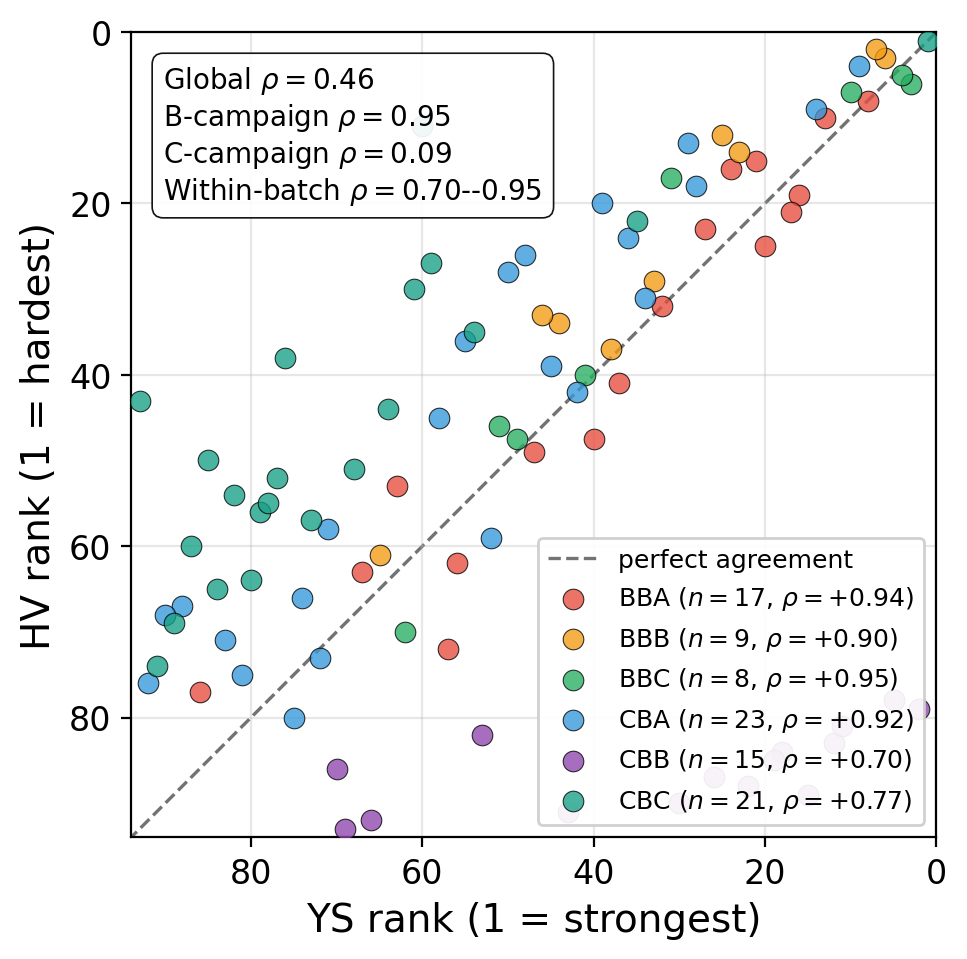
\includegraphics[width=0.6\textwidth]{fig_hv_ys_rank.png}
  \caption{HV rank versus YS rank across the 93 alloys, colored by batch. Per-batch correlations cluster along the diagonal ($\rho = 0.70$--$0.95$); the pooled ranking degrades to $\rho = 0.46$, with the processing-swept C-campaign at $\rho = 0.09$.}
  \label{fig:hv_rank}
\end{figure}

% ============================================================
\section{Model diagnostics and per-batch LOBO}
\label{si:diagnostics}

\subsection{M3 robustness}
A 1000-replicate Monte Carlo perturbation of grain sizes by their measured uncertainty shifts $\alpha_V$, $\alpha_\text{Co}$, $\alpha_\text{Cr}$, and $\alpha_\text{Fe}$ by less than $\pm 15\%$ and $k_\text{HP}$ by $\pm 39\%$.
A 10\,000-replicate bootstrap yields parameter SE ratios of 0.99--1.54 (bootstrap/OLS), indicating modest departures from normality but no instability.
Subset analysis gives V-containing $k_\text{HP} \approx 1269$ vs.\ V-free $\approx 299$~MPa$\cdot\mu$m$^{1/2}$ with overlapping confidence intervals, and Simpson's-paradox screening shows only 8\% attenuation of the V--YS correlation when controlling for $d^{-1/2}$ ($r = +0.64 \to r_\text{partial} = +0.59$).
The full M3 coefficient set (Table~\ref{tab:m3_coef}) is exported with standard errors and 95\% confidence intervals in the repository (\texttt{results/m3\_coefficients.csv}), together with fitted model pickles that reproduce every coefficient without re-running the analysis stack.

\begin{table}[htb]
\centering
\caption{Fitted M3 coefficients (Ni-solvent reference). The $\alpha_i$ are empirical regression weights for $\sigma_0$, not physics-based SSS contributions.}
\label{tab:m3_coef}
\small
\begin{tabular}{lcl}
\toprule
Parameter & Value & Interpretation \\
\midrule
$\sigma_{00}$ & 230~\si{MPa} & Intercept \\
$\alpha_V$    & $+291$ & V strongly raises $\sigma_0$ \\
$\alpha_{Mn}$ & $+82$  & Mn mildly raises $\sigma_0$ \\
$\alpha_{Al}$ & $-201$ & Al lowers $\sigma_0$ vs.\ Ni \\
$\alpha_{Co}$ & $-187$ & Co lowers $\sigma_0$ \\
$\alpha_{Cr}$ & $-308$ & Cr lowers $\sigma_0$ \\
$\alpha_{Cu}$ & $-334$ & Cu lowers $\sigma_0$ \\
$\alpha_{Fe}$ & $-360$ & Fe largest negative effect \\
$k_\text{HP}$ & $766$~MPa$\cdot\mu$m$^{1/2}$ & Constant across compositions \\
\bottomrule
\end{tabular}
\end{table}

\subsection{Hall--Petch slope: literature context}
Table~\ref{tab:khp_lit} places the fitted M3 slope among literature values for FCC alloys.
The grain-only global fit ($k_\text{HP} \approx 1149$~MPa$\cdot\mu$m$^{1/2}$) would sit above every literature entry except ordered Al$_{0.3}$CoCrFeNi; the composition-dependent intercept of M3 returns the slope to the middle of the FCC-HEA range, confirming that the inflation was an artifact of composition--slope confounding.

\begin{table}[htb]
\centering
\caption{Hall--Petch slope $k_\text{HP}$ in FCC alloys: literature comparison.}
\label{tab:khp_lit}
\small
\begin{tabular}{lcl}
\toprule
Alloy & $k_\text{HP}$ (MPa$\cdot\mu$m$^{1/2}$) & Reference \\
\midrule
Pure Cu                       & 110  & \cite{Cordero2016} \\
Pure Ni                       & 160  & \cite{Cordero2016} \\
316L stainless steel          & 322  & Singh et al.\ (2002) \\
CoCrFeMnNi                    & 494  & \cite{Otto2013} \\
CoCrFeNi                      & 516  & Yoshida et al.\ (2019) \\
CoCrNi                        & 265  & \cite{Yoshida2017} \\
This work (M3, 93 FCC HEAs)   & 766  & Global constant \\
Al$_{0.3}$CoCrFeNi (FCC)      & 824  & Gwalani et al.\ (2017) \\
Al$_{0.3}$CoCrFeNi (ordered)  & 1014 & Gwalani et al.\ (2017) \\
\bottomrule
\end{tabular}
\end{table}

\subsection{Per-batch LOBO}
Aggregate LOBO averages over folds of very different difficulty.
Table~\ref{tab:perbatch} breaks the LOBO score down by held-out batch for the classical HP baseline and M3, together with the composition-hull containment of each held-out batch by the training batches.
M3 improves on classical HP in every fold; the hardest folds (CBC, BBB) are exactly the least-covered batches.

\begin{table}[htb]
\centering
\caption{Per-batch LOBO $R^2$ with composition-hull containment of the held-out batch.}
\label{tab:perbatch}
\small
\begin{tabular}{lccccc}
\toprule
Held-out batch & $n_\text{test}$ & Hull cont. & HP $R^2$ & M3 $R^2$ & M3 RMSE \\
\midrule
BBA & 17 & 0.88 & 0.41 & 0.70 & 32.9 \\
BBB & 9  & 0.56 & 0.14 & 0.31 & 57.7 \\
BBC & 8  & 0.75 & 0.26 & 0.66 & 51.9 \\
CBA & 23 & 1.00 & 0.29 & 0.42 & 44.9 \\
CBB & 15 & 0.93 & 0.17 & 0.58 & 49.6 \\
CBC & 21 & 0.48 & $-0.04$ & 0.41 & 60.4 \\
\bottomrule
\end{tabular}
\end{table}

\bibliographystyle{elsarticle-num}
\bibliography{references}

\end{document}
